% Options for packages loaded elsewhere
\PassOptionsToPackage{unicode}{hyperref}
\PassOptionsToPackage{hyphens}{url}
\PassOptionsToPackage{dvipsnames,svgnames,x11names}{xcolor}
%
\documentclass[
  11pt,
  letterpaper,
  DIV=11,
  numbers=noendperiod]{scrartcl}

\usepackage{amsmath,amssymb}
\usepackage{setspace}
\usepackage{iftex}
\ifPDFTeX
  \usepackage[T1]{fontenc}
  \usepackage[utf8]{inputenc}
  \usepackage{textcomp} % provide euro and other symbols
\else % if luatex or xetex
  \usepackage{unicode-math}
  \defaultfontfeatures{Scale=MatchLowercase}
  \defaultfontfeatures[\rmfamily]{Ligatures=TeX,Scale=1}
\fi
\usepackage[]{lmodern}
\ifPDFTeX\else  
    % xetex/luatex font selection
\fi
% Use upquote if available, for straight quotes in verbatim environments
\IfFileExists{upquote.sty}{\usepackage{upquote}}{}
\IfFileExists{microtype.sty}{% use microtype if available
  \usepackage[]{microtype}
  \UseMicrotypeSet[protrusion]{basicmath} % disable protrusion for tt fonts
}{}
\makeatletter
\@ifundefined{KOMAClassName}{% if non-KOMA class
  \IfFileExists{parskip.sty}{%
    \usepackage{parskip}
  }{% else
    \setlength{\parindent}{0pt}
    \setlength{\parskip}{6pt plus 2pt minus 1pt}}
}{% if KOMA class
  \KOMAoptions{parskip=half}}
\makeatother
\usepackage{xcolor}
\usepackage[margin=1in,top=0.9in,bottom=0.9in]{geometry}
\setlength{\emergencystretch}{3em} % prevent overfull lines
\setcounter{secnumdepth}{5}
% Make \paragraph and \subparagraph free-standing
\makeatletter
\ifx\paragraph\undefined\else
  \let\oldparagraph\paragraph
  \renewcommand{\paragraph}{
    \@ifstar
      \xxxParagraphStar
      \xxxParagraphNoStar
  }
  \newcommand{\xxxParagraphStar}[1]{\oldparagraph*{#1}\mbox{}}
  \newcommand{\xxxParagraphNoStar}[1]{\oldparagraph{#1}\mbox{}}
\fi
\ifx\subparagraph\undefined\else
  \let\oldsubparagraph\subparagraph
  \renewcommand{\subparagraph}{
    \@ifstar
      \xxxSubParagraphStar
      \xxxSubParagraphNoStar
  }
  \newcommand{\xxxSubParagraphStar}[1]{\oldsubparagraph*{#1}\mbox{}}
  \newcommand{\xxxSubParagraphNoStar}[1]{\oldsubparagraph{#1}\mbox{}}
\fi
\makeatother


\providecommand{\tightlist}{%
  \setlength{\itemsep}{0pt}\setlength{\parskip}{0pt}}\usepackage{longtable,booktabs,array}
\usepackage{calc} % for calculating minipage widths
% Correct order of tables after \paragraph or \subparagraph
\usepackage{etoolbox}
\makeatletter
\patchcmd\longtable{\par}{\if@noskipsec\mbox{}\fi\par}{}{}
\makeatother
% Allow footnotes in longtable head/foot
\IfFileExists{footnotehyper.sty}{\usepackage{footnotehyper}}{\usepackage{footnote}}
\makesavenoteenv{longtable}
\usepackage{graphicx}
\makeatletter
\newsavebox\pandoc@box
\newcommand*\pandocbounded[1]{% scales image to fit in text height/width
  \sbox\pandoc@box{#1}%
  \Gscale@div\@tempa{\textheight}{\dimexpr\ht\pandoc@box+\dp\pandoc@box\relax}%
  \Gscale@div\@tempb{\linewidth}{\wd\pandoc@box}%
  \ifdim\@tempb\p@<\@tempa\p@\let\@tempa\@tempb\fi% select the smaller of both
  \ifdim\@tempa\p@<\p@\scalebox{\@tempa}{\usebox\pandoc@box}%
  \else\usebox{\pandoc@box}%
  \fi%
}
% Set default figure placement to htbp
\def\fps@figure{htbp}
\makeatother

\usepackage{amsmath}
\usepackage{amsthm}
\usepackage{amssymb}
\usepackage{amsfonts}
\usepackage{booktabs}
\usepackage{setspace}
\usepackage{graphicx}
\usepackage{algorithm}
\usepackage[noend]{algpseudocode}
% Define math operators if needed
\DeclareMathOperator*{\argmax}{arg\,max}
\DeclareMathOperator*{\Exp}{\mathbb{E}} % Expectation operator
\newcommand{\sym}[1]{\ensuremath{^{#1}}}
\KOMAoption{captions}{tableheading}
\makeatletter
\@ifpackageloaded{caption}{}{\usepackage{caption}}
\AtBeginDocument{%
\ifdefined\contentsname
  \renewcommand*\contentsname{Table of contents}
\else
  \newcommand\contentsname{Table of contents}
\fi
\ifdefined\listfigurename
  \renewcommand*\listfigurename{List of Figures}
\else
  \newcommand\listfigurename{List of Figures}
\fi
\ifdefined\listtablename
  \renewcommand*\listtablename{List of Tables}
\else
  \newcommand\listtablename{List of Tables}
\fi
\ifdefined\figurename
  \renewcommand*\figurename{Figure}
\else
  \newcommand\figurename{Figure}
\fi
\ifdefined\tablename
  \renewcommand*\tablename{Table}
\else
  \newcommand\tablename{Table}
\fi
}
\@ifpackageloaded{float}{}{\usepackage{float}}
\floatstyle{ruled}
\@ifundefined{c@chapter}{\newfloat{codelisting}{h}{lop}}{\newfloat{codelisting}{h}{lop}[chapter]}
\floatname{codelisting}{Listing}
\newcommand*\listoflistings{\listof{codelisting}{List of Listings}}
\makeatother
\makeatletter
\makeatother
\makeatletter
\@ifpackageloaded{caption}{}{\usepackage{caption}}
\@ifpackageloaded{subcaption}{}{\usepackage{subcaption}}
\makeatother

\usepackage{bookmark}

\IfFileExists{xurl.sty}{\usepackage{xurl}}{} % add URL line breaks if available
\urlstyle{same} % disable monospaced font for URLs
\hypersetup{
  pdftitle={The Great Re-Valuation: Preferences, Technology, and the Rise of Remote Work},
  pdfauthor={Mitchell Valdes-Bobes; Anna Lukianova},
  colorlinks=true,
  linkcolor={blue},
  filecolor={Maroon},
  citecolor={Blue},
  urlcolor={Blue},
  pdfcreator={LaTeX via pandoc}}


\title{The Great Re-Valuation: Preferences, Technology, and the Rise of
Remote Work}
\author{Mitchell Valdes-Bobes \and Anna Lukianova}
\date{August 31, 2025}

\begin{document}
\maketitle
\begin{abstract}
Write the final abstract based on the estimated results. Should cover:
Motivation (post-pandemic shift), Question (Preferences vs.~Technology),
Method (Structural search model with heterogeneity), Estimation (SMM on
2019 vs.~2024), Key Finding (Preference shock dominates), and
Contribution (Structural decomposition).
\end{abstract}


\setstretch{1.5}
\section{Introduction}\label{introduction}

he COVID-19 pandemic reshaped the landscape of work almost overnight,
catapulting remote and hybrid work arrangements from niche to
mainstream. By 2024, nearly 30\% of U.S. workdays were performed
remotely---over four times the pre-pandemic share
(\textcolor{green}{Barrero, Bloom, and Davis, 2023}). This dramatic
shift presents a puzzle: while remote work is clearly valued by workers,
it has not led to a universal wage penalty, and the productivity
implications remain ambiguous.

Our research question is straightforward: to what extent did the recent
``great re-valuation'' of remote work stem from shifts in worker
preferences versus advances in technology? And how does the pattern of
matching between workers and firms help explain the observed patterns in
wages and work arrangements?

To answer these questions, we develop and estimate a general equilibrium
search model with heterogeneity in worker skills, firm remote-work
efficiency, and idiosyncratic worker tastes. A key innovation of our
empirical approach is a novel, continuous measure of occupational
teleworkability, which we construct using machine learning techniques.
This index allows for a more nuanced identification of firm-level remote
efficiency and sorting patterns than the binary measures used in prior
work \textcolor{green}{CITE}. We estimate the model's parameters using
the Simulated Method of Moments (SMM) on rich microdata from 2019 and
2024 to quantify the relative contributions of preference and technology
shocks. Our estimates reveal that the primary driver of the shift to
remote work has been

\line(1,0)\{250\}

\textbf{Case 1: Preferences Dominate}

\textcolor{red}{a profound re-valuation of in-office time by workers. We estimate a $X\%$ increase in the parameter governing the disutility of commuting and in-office presence, an effect that is over $N$ times larger than the concurrent $Y\%$ increase we estimate in the parameter for remote work technology. This indicates that the "great re-valuation" is fundamentally a story about evolving worker preferences, which reshaped the equilibrium sorting of workers to firms and the resulting wage and work arrangements.}

\line(1,0)\{250\}

\textbf{Case 2: Technology Dominates}

\textcolor{blue}{a significant technological shock that enhanced the viability of remote work. We estimate a $X\%$ increase in the parameter governing the relative productivity of remote technology, an effect that is over $N$ times larger than the modest $Y\%$ shift we estimate in the parameter for worker preferences. This suggests that the "great re-valuation" is fundamentally a story about technological adoption, which reshaped the equilibrium sorting of workers to firms and the resulting wage and work arrangements.}

\line(1,0)\{250\}

\section{Data and Stylized Facts of the Post-Pandemic Labor
Market}\label{data-and-stylized-facts-of-the-post-pandemic-labor-market}

\subsection{\texorpdfstring{\textbf{Empirical Evidence: Three Puzzles
Motivating a Structural
Approach}}{Empirical Evidence: Three Puzzles Motivating a Structural Approach}}\label{empirical-evidence-three-puzzles-motivating-a-structural-approach}

\begin{itemize}
\tightlist
\item
  {[}cite\_start{]}\textbf{Narrative Introduction (Revised):}
  \emph{(Applying the ``Punchline First'' principle {[}cite: 55,
  231{]})} Start by stating the section's main conclusion directly. For
  example: ``This section presents three key empirical puzzles of the
  post-pandemic labor market. First, the adoption of flexible work is
  highly stratified by education and occupation. Second, wages exhibit a
  complex, concave relationship with an occupation's potential for
  remote work, even after conditioning on rich observable
  characteristics. Third, we document powerful sorting between highly
  educated workers and remote-friendly occupations. We argue that these
  facts, taken together, are difficult to reconcile with a simple
  framework and point toward a deeper sorting mechanism based on latent
  worker skill. This evidence forms the empirical foundation that our
  structural model is designed to explain. Our analysis primarily relies
  on data from the Current Population Survey (CPS).''
\end{itemize}

\begin{center}\rule{0.5\linewidth}{0.5pt}\end{center}

\subsubsection{\texorpdfstring{\textbf{Data, Sample Construction, and
Limitations}}{Data, Sample Construction, and Limitations}}\label{data-sample-construction-and-limitations}

\begin{itemize}
\tightlist
\item
  {[}cite\_start{]}\textbf{Goal:} Describe the data, sample selection,
  and transparently address any limitations to build credibility{[}cite:
  209{]}.
\item
  \textbf{Content:}

  \begin{itemize}
  \tightlist
  \item
    \textbf{Data Source:} Describe the Current Population Survey (CPS),
    the supplements used (e.g., ASEC), and the sample years (e.g., 2019,
    2022-2024).
  \item
    {[}cite\_start{]}\textbf{Justification and Limitations:} \emph{(New
    subsection to boost credibility )} Briefly explain \emph{why} the
    CPS is the appropriate dataset for this analysis (e.g., large sample
    size, detailed demographics). Then, be transparent about its
    limitations (e.g., ``We acknowledge that the CPS questions on remote
    work are self-reported and may contain measurement error.
    Furthermore, our wage measure does not include non-wage benefits,
    which may be an important margin of adjustment.'').
  \item
    \textbf{Sample Selection:} Detail the filters applied to the raw
    data (e.g., full-time workers, age 25-64, non-military, etc.).
  \item
    {[}cite\_start{]}\textbf{Table 1: Summary Statistics of the Analysis
    Sample (2024):} \emph{(Title revised to be more descriptive {[}cite:
    247{]})}

    \begin{itemize}
    \tightlist
    \item
      \textbf{Content:} Present weighted means and standard deviations
      for key variables (age, education, log wage, shares by sex/race).
    \item
      {[}cite\_start{]}\textbf{Notes:} \emph{(Ensure the table is
      self-contained {[}cite: 243{]}{[}cite\_start{]})} The notes should
      define all variables, state the data source (CPS ASEC), and
      specify the sample restrictions and application of survey weights,
      ensuring replicability{[}cite: 197{]}.
    \end{itemize}
  \end{itemize}
\end{itemize}

\begin{center}\rule{0.5\linewidth}{0.5pt}\end{center}

\subsubsection{\texorpdfstring{\textbf{Measuring Occupational
Amenability to Remote Work
(\(\psi\))}}{Measuring Occupational Amenability to Remote Work (\textbackslash psi)}}\label{measuring-occupational-amenability-to-remote-work-psi}

\begin{itemize}
\tightlist
\item
  \textbf{Goal:} Introduce the key explanatory variable (\(\psi\)) and
  document its strong correlation with other key worker and job
  characteristics, highlighting the primary empirical challenge.
\item
  \textbf{Narrative:} Explain that a quantitative measure of an
  occupation's intrinsic suitability for remote work is needed.
\item
  \textbf{Construction of \(\psi\):}

  \begin{itemize}
  \tightlist
  \item
    \textbf{Methodology:} Briefly explain the construction methodology
    (e.g., following Dingel and Neiman (2020)).
  \item
    \textbf{Interpretation:} State clearly that \(\psi\) is a continuous
    {[}0, 1{]} index.
  \end{itemize}
\item
  \textbf{Figure 1: The Skewed Distribution of Remote-Work Potential:}
  \emph{(Title revised for clarity)}

  \begin{itemize}
  \tightlist
  \item
    \textbf{Content:} A density plot of the \(\psi\) index across
    occupations, weighted by employment.
  \item
    \textbf{Takeaway:} Emphasize the concentration, e.g., ``The
    potential for remote work is a scarce occupational feature. Over
    half of all workers are in occupations with \(\psi < 0.2\).''
  \end{itemize}
\item
  \textbf{Table 2: Worker and Job Characteristics by \(\psi\) Quantile:}

  \begin{itemize}
  \tightlist
  \item
    \textbf{Content:} Show average education, wages, and industry
    composition for workers in Low-\(\psi\), Mid-\(\psi\), and
    High-\(\psi\) occupations.
  \item
    {[}cite\_start{]}\textbf{Takeaway and Narrative Framing:} Frame this
    table as demonstrating the core challenge of confounding
    variables{[}cite: 221{]}. State clearly: ``This table reveals the
    central empirical challenge that motivates our structural approach.
    High-\(\psi\) occupations are not randomly assigned; they are
    disproportionately held by higher-educated workers in higher-paying
    industries. This demonstrates that simple OLS regressions of wages
    on remote work status would be severely biased by worker and firm
    selection.''
  \end{itemize}
\end{itemize}

\begin{center}\rule{0.5\linewidth}{0.5pt}\end{center}

\subsubsection{\texorpdfstring{\textbf{The Three
Puzzles}}{The Three Puzzles}}\label{the-three-puzzles}

\begin{itemize}
\item
  \textbf{Goal:} Present the key empirical patterns as distinct puzzles
  that the model must explain. {[}cite\_start{]}This turns the section
  into a compelling narrative{[}cite: 359{]}.
\item
  \textbf{Puzzle 1: The Stratification of Work Arrangements.} 🔎

  \begin{itemize}
  \tightlist
  \item
    \textbf{Figure 2: The Post-Pandemic Rise of Hybrid and Remote Work:}
    Time-series plot (2019-2024) of In-Person, Hybrid, and Full-Remote
    work shares.
  \item
    \textbf{Figure 3: Remote and Hybrid Work are Dominated by the Highly
    Educated in High-\(\psi\) Jobs:} The two-panel bar chart.
  \item
    \textbf{Narrative:} ``The first puzzle is the sharp stratification
    of who performs flexible work. It is not a widespread phenomenon but
    one concentrated in a specific corner of the labor market.''
  \end{itemize}
\item
  \textbf{Puzzle 2: The Concave Wage Profile.} 📈

  \begin{itemize}
  \tightlist
  \item
    \textbf{Figure 4: The Non-Linear Relationship Between Wages and
    Occupational Flexibility:} Binned scatter plot of residual log wage
    against your \(\psi\) or \(\alpha\) index.
  \item
    \textbf{Table 3: OLS and Fixed-Effects Estimates of the
    Wage-\(\psi\) Profile:} The key regression table showing \(\psi\)
    (positive) and \(\psi^2\) (negative) coefficients.
  \item
    \textbf{Narrative:} ``The second puzzle lies in the wage structure.
    After controlling for an extensive set of worker and job
    characteristics, we find a positive but concave relationship between
    wages and an occupation's remote-work potential. This suggests a
    premium that diminishes at higher levels, a pattern that simple
    theories of compensating differentials struggle to explain.''
  \end{itemize}
\item
  \textbf{Puzzle 3: Powerful Sorting on Unobservables.} 🧩

  \begin{itemize}
  \tightlist
  \item
    \textbf{Figure 5: Strong Assortative Matching on Education:} Scatter
    plot showing the positive correlation between worker education and
    their occupation's average \(\psi\).
  \item
    \textbf{Table 4: Evidence of a Sorting Premium:} \emph{(Revised
    framing)} Your key regression table.
  \item
    \textbf{Narrative Framing:} Be precise about what this regression
    shows. ``The final puzzle points to the importance of unobserved
    factors. The strong positive sorting between worker education and
    occupational \(\psi\) is striking. More importantly, even
    \emph{within the subsample of workers in flexible jobs}, we find a
    significant wage premium associated with being in a high-\(\psi\)
    occupation after controlling for education (Table 4). This is not a
    causal estimate of a `return to \(\psi\),' but rather evidence
    consistent with a sorting mechanism where higher-skilled workers
    (both observably and unobservably) sort into high-\(\psi\) jobs.
    This is the final piece of evidence our model must rationalize.''
    {[}cite\_start{]}This framing shows intellectual honesty and clearly
    defines the purpose of the regression{[}cite: 223{]}.
  \end{itemize}
\end{itemize}

\begin{center}\rule{0.5\linewidth}{0.5pt}\end{center}

\subsubsection{\texorpdfstring{\textbf{Synthesizing the Puzzles and
Motivating the Structural
Model}}{Synthesizing the Puzzles and Motivating the Structural Model}}\label{synthesizing-the-puzzles-and-motivating-the-structural-model}

\begin{itemize}
\tightlist
\item
  \textbf{Goal:} Summarize and make the case for your model.
\item
  \textbf{Narrative:} Your original paragraph is excellent and already
  aligns perfectly with the guide's principles. It masterfully
  summarizes the puzzles and pivots to the solution. I would only
  suggest a slightly more active title for the subsection.
  \textgreater{} ``The empirical evidence points to a complex new
  equilibrium. Remote work is concentrated among the highly educated in
  specific occupations and is associated with a positive, concave wage
  profile that persists after controlling for these observable
  characteristics. The strong assortative matching suggests the presence
  of a deeper, unobserved factor driving these patterns. To
  simultaneously rationalize the distribution of work arrangements, the
  complex wage structure, and the powerful sorting dynamics, we develop
  and estimate a structural search model. The model's central mechanism
  is the interaction between a latent, continuously distributed worker
  skill, \(h\), and the observable occupational technology, \(\psi\),
  which jointly determine productivity, wages, and the choice of
  workplace flexibility.''
\end{itemize}

\section{A Model of Labor Search with Heterogeneous Preferences for
Workplace
Flexibility}\label{a-model-of-labor-search-with-heterogeneous-preferences-for-workplace-flexibility}

\textcolor{green}{Statement of purpose...}

We consider a labor market populated by a continuum of firms and
infinitely lived, risk-neutral workers. This framework abstracts from
life-cycle and precautionary savings motives to focus solely on the
trade-offs inherent in job search and workplace arrangements.
Heterogeneity is central to our analysis: workers differ in their skill
level, \(h \in \mathcal{H}\), which determines their baseline
productivity, while firms differ in their remote work efficiency,
\(\psi \in \Psi\). This parameter primarily reflects occupation-level
characteristics that determine a job's suitability for remote work, but
it also encompasses firm-specific factors like technological
infrastructure and organizational capacity.

The measure of unemployed workers of skill level \(h\) is denoted
\(u(h)\), creating an aggregate stock of job seekers
\(L=\int_{\mathcal{H}}u(h)dh\). Similarly, the measure of vacancies
posted for type-\(\psi\) jobs is \(v(\psi)\), which aggregates to a
total of \(V=\int v(\psi)d\psi\) job opportunities. This supply of
vacancies is determined by a free-entry condition, where firms can
create and post jobs a cost \(\kappa(v)\), doing so until the expected
value of filling a position equals the cost of posting. Looking for a
job is a time consuming effort, something we characterized by assuming
search and matching frictions. A standard constant-returns-to-scale
matching function, \(M(L,V)\), governs the meeting process between
unemployed workers and vacancies. This process determines the key
outcomes of the search process: the job-finding rate for workers,
\(p(\theta)\), and the vacancy-filling rate for firms, \(q(\theta)\),
both of which depend on the aggregate labor market tightness,
\(\theta = V/L\).

\textbf{Worker preferences} over wage and remote work bundles
\(\{(w, \alpha)\}_{\mathbb{R}_{+}\times[0,1]}\) continuously
differentiable and concave to ensure well-behaved optimization. We make
two standard assumptions: utility is strictly increasing in wages
(\(u_w > 0\)), as workers prefer more consumption, and it is also
increasing in the remote work share (\(u_\alpha > 0\)), reflecting the
direct value workers place on the flexibility and amenities associated
with working from home.

A key assumption governs the trade-off between these two goods: we
assume the Marginal Rate of Substitution remote work and wages:
\(MRS_{\alpha,w} = u_\alpha / u_w\), is \emph{increasing} in \(\alpha\).
In economic terms, this means that as a worker's remote share increases,
they require progressively larger wage compensation to give up an
additional unit of remote work. This non-standard assumption is designed
to capture real-world phenomena that can lead to a preference for corner
solutions (either fully in-person or fully remote). For example, it can
reflect significant lifestyle adjustments that make a fully remote setup
particularly valuable once established, or the presence of high fixed
costs (e.g., commuting, separate childcare arrangements) associated with
even a single day of in-office presence, which can make hybrid schedules
less
desirable.\textcolor{green}{THERE IS DATA IN SWAA TO BACK THIS UP SHOULD HAVE A FOOTNOTE HERE.}

\textbf{The Production technology} \(Y\), depends on the remote work
share \(\alpha\), the worker's skill \(h\), and the firm/occupation's
remote conduciveness \(\psi\). The production function takes the form of
a linear combination of output from in-person and remote work:
\begin{equation}\phantomsection\label{eq-prod-fun}{Y(\alpha \mid \psi, h) = A(h) \cdot \left((1 - \alpha) + \alpha \cdot g(h, \psi)\right)}\end{equation}
Here, \(A(h)=A_0 + A_1 h\) is the baseline output of a worker with skill
\(h\) in a fully in-person setting, with \(A'(h) > 0\). Notice that the
only source of heterogeneity on the firm side is the parameter \(\psi\),
which captures the firm's remote work efficiency, therefore for full-in
person arrangements \((\alpha = 0)\), the sole determinant of output is
worker skill.

Remote work productivity is scaled by an efficiency adjustment factor,
\(g(h, \psi)\), which we specify with a flexible functional form:
\begin{equation}\phantomsection\label{eq-remote-prod}{g(h, \psi) = \psi_0 \cdot h^\phi \cdot \psi^\nu}\end{equation}
n this specification, \(\psi_0\)\hspace{0pt} is a baseline technology
parameter for remote productivity across the economy, while \(\phi\) and
\(\nu\) are the output elasticities with respect to worker skill and
firm remote work efficiency respectively. We assume \(\psi>0\) and
\(\nu>0\). The assumption that remote productivity increases with worker
skill (\(\phi>0\)) is motivated by the idea that higher-skilled workers
often engage in tasks requiring greater autonomy and
self-direction---traits that are highly complementary to the remote work
environment. Furthermore, their work may be less reliant on physical
co-location for supervision and execution compared to more routine
tasks.

Crucially, this functional form implies a positive cross-partial
derivative \((g_{h\psi}​>0)\), meaning there is a
\textbf{complementarity} between worker skill and firm remote
efficiency. This complementarity is the central force that will drive
assortative matching in the model, creating a tendency for high-skill
workers to sort into firms that are most efficient at remote work.

\subsection{Deterministic Choice of Flexibility: A
Benchmark}\label{deterministic-choice-of-flexibility-a-benchmark}

To build intuition for the core trade-offs governing workplace
flexibility, we first analyze a simplified benchmark model where the
choice of work arrangement is \textbf{fully deterministic}. This
approach allows us to isolate the fundamental economic forces driven by
technology and preferences before we introduce additional sources of
heterogeneity.

For any given work arrangement, \(\alpha\), the total flow surplus of a
match is the sum of the firm's profit and the worker's utility. The
firm's per-period profit is its output net of the wage paid,
\(\Pi(h, \psi \mid w, \alpha)=Y(h, \psi\mid \alpha)−w\). The worker's
utility, given our quasi-linear specification, is their wage net of the
non-pecuniary cost of in-office work, \(u(w, \alpha)=w−c(1−\alpha)\).
The joint surplus, \(J(\alpha)\), is therefore:
\begin{equation}\phantomsection\label{eq-surplus-alpha}{\pi(h, \psi \mid \alpha) = \Pi(h, \psi \mid w, \alpha) +  u(w, \alpha )= \Big(Y(h, \psi \mid \alpha) - w\Big) + \Big(w - c(1-\alpha)\Big)}\end{equation}
As the wage, \(w\), is a pure intra-match transfer, it cancels out. This
leaves the joint surplus dependent only on the match's total output and
the worker's non-pecuniary cost.

We assume the wage is determined by generalized Nash bargaining between
the firm and the worker. This bargaining framework implies that the
match operates under an \textbf{efficient contract}, which separates the
problem into two parts: an efficiency decision and a distributional
decision. First, the remote work share, \(\alpha\) is chosen jointly to
maximize the total surplus generated by the match. Second, this
maximized surplus is divided between the worker and the firm according
to their exogenous bargaining power \(\xi\). With our choice of
quasi-linear utility, the wage acts as the endogenous transfer that
facilitates this division. This efficient contracting structure allows
us to solve for the optimal work arrangement by first focusing on the
joint surplus maximization given by equation
Equation~\ref{eq-surplus-alpha}:
\begin{equation}\phantomsection\label{eq-surplus-max}{\pi = \max_{\alpha \in [0,1]} \quad \Big\{ Y(\alpha \mid \psi, h) - c(\alpha)\Big\}}\end{equation}

The solution to problem Equation~\ref{eq-surplus-max} reveals that the
optimal work arrangement, \(\alpha^∗(\psi,h)\), partitions the market
into three distinct regimes based on the firm's remote efficiency
\(\psi\), , relative to two skill-dependent thresholds,
\(\underline{\psi}(h)\) and \(\overline{\psi}(h)\):
\begin{equation}\phantomsection\label{eq-optimal-alpha-deterministic}{\alpha^{*}(\psi,h) = \begin{cases}
    0 & \text{if } \psi \leq \underline{\psi}(h) \quad \text{(Full In-Person)} \\ 
    1 - \left[ \frac{A_1h(1 - g(\psi,h))}{c_0} \right]^{\frac{1}{\chi}} & \text{if } \underline{\psi}(h) < \psi < \overline{\psi}(h) \quad \text{(Hybrid)} \\
    1 & \text{if } \psi \geq \overline{\psi}(h) \quad \text{(Full Remote)}
\end{cases}}\end{equation}

These thresholds represent economic tipping points where the trade-off
between \textbf{production efficiency and worker amenities} dictates the
optimal work arrangement. The worker always values the non-pecuniary
benefits of remote work, while the firm is focused on the impact on
output, which may be positive or negative.

\begin{itemize}
\tightlist
\item
  For firms with low remote efficiency
  (\(\psi\leq\underline{\psi}​(h)\)), the \textbf{productivity loss} from
  remote work is too severe. Although the worker desires the remote work
  amenity, the firm cannot afford to grant this preference because the
  marginal drop in output is greater than the worker's marginal
  valuation for it. Thus, the match defaults to a fully in-person
  arrangement.
\item
  Conversely, for firms with very high efficiency
  (\(\psi\geq\overline{\psi}(h)\)), remote work may be so productive
  that it generates a \textbf{``productivity premium.''} In this
  scenario, maximizing output and satisfying the worker's desire for
  remote work are aligned, making a fully remote arrangement the optimal
  choice for the match.
\item
  \textbf{Hybrid work} emerges for the intermediate firms where a clear
  trade-off exists. These firms are willing to ``sell'' the remote work
  amenity to the worker, accepting a modest productivity loss (or
  smaller gain) up to the point where the marginal cost in terms of
  output exactly equals the worker's marginal non-pecuniary benefit.
\end{itemize}

\begin{figure}

\centering{

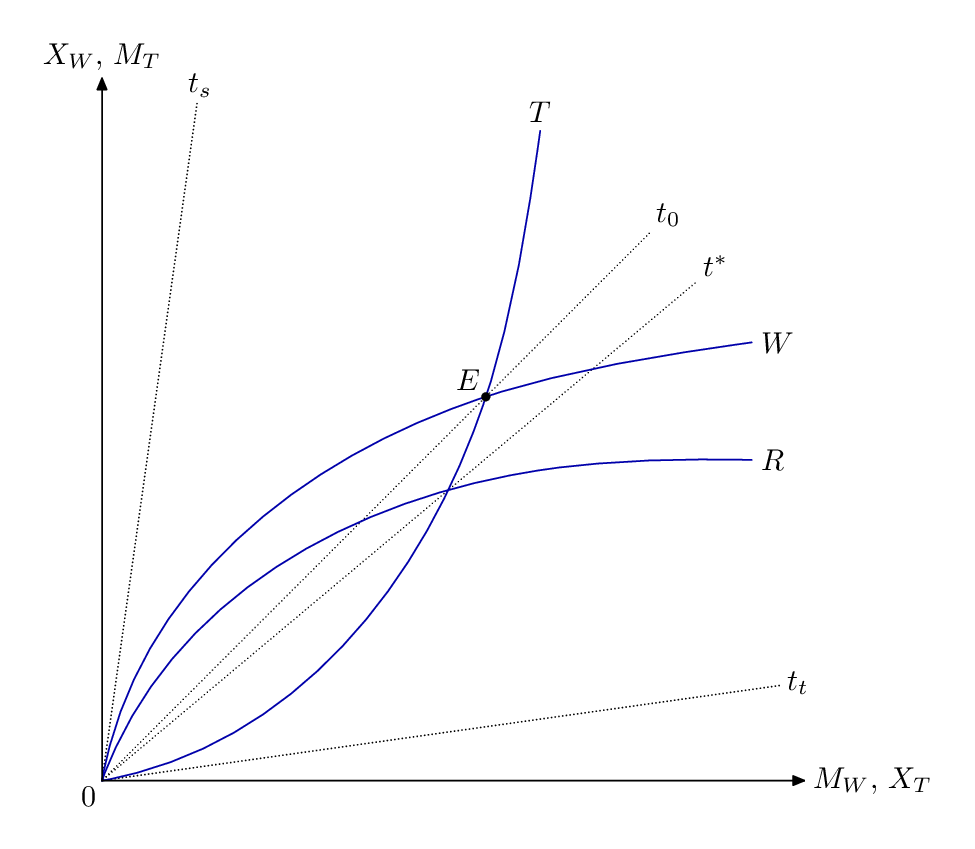
\includegraphics[width=0.8\linewidth,height=\textheight,keepaspectratio]{../figures/stock_image.png}

}

\caption{\label{fig-deterministic-thresholds}Optimal Work Arrangements
in the Deterministic Benchmark. The figure illustrates how the optimal
remote work share, \(\alpha^*\), depends on worker skill (\(h\)) and
firm remote efficiency (\(\psi\)). The market is partitioned into three
regimes by two skill-dependent thresholds, \(\underline{\psi}(h)\) and
\(\overline{\psi}(h)\). Matches falling below the lower threshold are
fully in-person, matches above the upper threshold are fully remote, and
matches between the thresholds adopt a hybrid arrangement.}

\end{figure}%

This deterministic model provides sharp predictions: for any given
worker, only firms within a specific range of remote efficiency will
offer a hybrid arrangement. However, this stark segmentation is at odds
with the smooth distribution of work arrangements observed in the data.
This motivates the introduction of idiosyncratic preferences, which
allows for a richer and more realistic pattern of matching.

\subsection{The Full Model with Idiosyncratic
Preferences}\label{the-full-model-with-idiosyncratic-preferences}

The deterministic benchmark provides sharp predictions but cannot
account for the smooth distribution of work arrangements observed in the
data. To capture this rich heterogeneity, we extend the model by
introducing idiosyncratic worker preferences. We posit that a worker
only discovers their true preference for a specific work arrangement
after a match is formed. Factors such as the actual commute, the
specific in-office culture, or the suitability of their home environment
for work are not fully known ex-ante. This uncertainty is captured by an
idiosyncratic taste shock.

For a given contract ( \(w, \alpha\) ), a worker's realized utility is
the sum of their deterministic utility and this stochastic taste shock:
\begin{equation}\phantomsection\label{eq-utility-random}{u(w, \alpha ; \varepsilon)=w-c(1-\alpha)+\mu \cdot \varepsilon(\alpha)}\end{equation}
Here, \(\varepsilon(\alpha)\) is the realization of the taste shock for
a remote share \(\alpha\), and \(\mu\) is a scale parameter governing
its importance. Analogous to the deterministic model, the total
\textbf{realized joint surplus} for a given arrangement and taste shock,
is the sum of the firm's profit and the worker's realized utility. The
wage remains a pure transfer and cancels out, leaving the surplus
dependent only on the physical aspects of the match and the worker's
non-pecuniary utility. Following the discrete choice literature, we
assume \(\varepsilon(\alpha)\) follows a Type I Extreme Value (Gumbel)
process.

Before the idiosyncratic taste shocks are realized, the firm and worker
jointly maximize the expected value of their match. This value, known as
the ``inclusive value,'' accounts for the option to choose the best
possible work arrangement once the shocks are revealed. The ex-ante
joint maximization problem is:

\begin{equation}\phantomsection\label{eq-flow-value-expected}{\pi(h, \psi)  = \max_{\alpha \in [0,1]} \mathbb{E}_{\varepsilon} \left[ \underbrace {Y(\alpha \mid \psi, h) - c(\alpha)}_{V(h, \psi \mid \alpha)} + \mu \cdot \varepsilon(\alpha) \right]}\end{equation}

Where \(V(h, \psi; \alpha)\) denote the deterministic component of the
joint value of the match. A well-known result from the discrete choice
literature is that when the shocks \(\varepsilon(\alpha)\) are drawn
from a Type I Extreme Value (Gumbel) distribution, this maximization
problem has a convenient closed-form solution. The maximized expected
surplus of the match is given by the log-sum integral:

\begin{equation}\phantomsection\label{eq-flow-value-solved}{\pi(h, \psi) = \mu \ln \left( \int_0^1 \exp\left(\frac{V(h, \psi; \alpha)}{\mu}\right) d\alpha \right)}\end{equation}

This inclusive value is the fundamental object that enters the
equilibrium Bellman equations that we define next. We define the flow
surplus of the match, \(s(h,\psi)\), as this value net of the worker's
outside option, their flow unemployment benefit \(b(h)\):

\begin{equation}\phantomsection\label{eq-flow-surplus}{ s(h, \psi) = \left[ \mu \ln \left( \int_0^1 \exp\left(\frac{V(h, \psi; \alpha)}{\mu}\right) d\alpha \right) \right] - b(h)}\end{equation}

This expected flow surplus, \(s(h,\psi)\), is the fundamental object
that determines the value of a match in the full equilibrium.

A direct consequence of this framework is that the choice of \(\alpha\)
becomes probabilistic. The probability that a specific arrangement
\(\alpha\) is chosen for a match \((h, \psi)\) follows the continuous
logit formula:

\begin{equation}\phantomsection\label{eq-prob-alpha}{ p(\alpha \mid h, \psi) = \frac{\exp\left({V(h, \psi; \alpha)}{\mu^{-1}}\right)}{\int_0^1 \exp\left({V(h, \psi; a)}{\mu^{-1}}\right) da} }\end{equation}

This structure provides the link between the two versions of the model:
the hard thresholds of the deterministic benchmark now become the
central inflection points of the smooth choice probabilities in the full
model. The scale parameter, \(\mu\), governs how ``blurry'' or ``soft''
these thresholds are.

\subsection{Equilibrium}\label{equilibrium}

A steady-state equilibrium is characterized by a set of value functions
for workers and firms, optimal vacancy posting by firms, and worker
flows that are balanced. These components are mutually consistent and
determine the aggregate state of the labor market. \#\#\# Value
Functions and Surplus

The equilibrium is defined by the lifetime values for workers and firms
in different states. We begin by defining the value of an ongoing match
and the value of unemployment, and from these, we derive the Bellman
equation for the match surplus, \(S(h,\psi)\), which will be shown to be
the central object that characterizes the equilibrium.

The joint value of a match, \(J(h, \psi)\), is the present discounted
value of all future returns. It is composed of the current period's
expected flow surplus, \(s(h,\psi)+b(h)\), plus the discounted
continuation value. With probability \((1-\delta)\), the match survives
and retains its value, and with probability \(\delta\), it is destroyed
and the worker's value reverts to that of unemployment,
\(U(h)\)\footnote{We assume that free entry make the value for a firm of
  a dicontinued match equal to zero}. This gives the Bellman equation:
\begin{equation}\phantomsection\label{eq-value-match}{ J(h, \psi) = \left( \pi(h,\psi) - b(h) \right) + \beta \left[ (1-\delta)J(h,\psi) + \delta U(h) \right] }\end{equation}
The value of unemployment for a worker of type \(h\), \(U(h)\), consists
of the current flow benefit, \(b(h)\), plus the expected value from job
search. With probability \(p(\theta)\), the worker contacts a firm, and
with probability \((1-p(\theta))\), they remain unemployed. The value of
a new match to a worker, \(W(h,\psi')\), is determined by our
\textbf{Nash bargaining} assumption, which dictates that the worker
receives their outside option, \(U(h)\), plus a share \(\xi\) of the
total match surplus, \(S(h, \psi')\). A match is only formed if the
surplus is positive. This gives the Bellman equation for unemployment:
\begin{equation}\phantomsection\label{eq-value-unemployment}{ U(h) = b(h) + \beta \left[ p(\theta)\mathbb{E}_{\psi'}\left[\max\{W(h,\psi'), U(h)\}\right] + (1-p(\theta))U(h) \right] }\end{equation}

Substituting \(W(h, \psi') = U(h) + \xi S(h, \psi')\) and simplifying
yields:
\begin{equation}\phantomsection\label{eq-value-unemployment-simplified}{ U(h) = b(h) + \beta U(h) + \beta p(\theta)\xi \int \max\{0, S(h,\psi')\} d\Gamma_v(\psi') }\end{equation}
The total match surplus is the net value created by the match, defined
as \(S(h, \psi) \equiv J(h, \psi) - U(h)\). We can derive its Bellman
equation by subtracting the equation for \(U(h)\) from the one for
\(J(h, \psi)\), which after rearranging highlights that the worker's
expected gain from search acts as an effective opportunity cost for the
match:
\begin{equation}\phantomsection\label{eq-value-surplus}{ S(h, \psi) = s(h, \psi) + \beta(1-\delta)S(h,\psi) - \beta p(\theta)\xi \int \max\{0, S(h,\psi')\} d\Gamma_v(\psi') }\end{equation}
Solving for \(S(h, \psi)\) gives the final expression:
\begin{equation}\phantomsection\label{eq-value-surplus-solved}{ S(h, \psi) = \frac{s(h, \psi) - \beta p(\theta) \xi \int \max\{0, S(h,\psi')\} d\Gamma_{v}(\psi')}{1 - \beta(1 - \delta)} }\end{equation}

This derivation highlights a key insight: the surplus equation is the
only object needed to solve for the equilibrium. Because the term
\(\max\{0, S(h,\psi')\}\) appears inside the integral, the sign of the
surplus itself determines the set of viable matches that will form. A
negative surplus means the parties are better off separated, and no
match is created. Therefore, \(S(h,\psi)\) is a sufficient statistic
that fully encodes the equilibrium matching decisions.

\subsubsection{Vacancy Creation and Market
Tightness}\label{vacancy-creation-and-market-tightness}

The number of vacancies is determined by firms' profit maximization.
Firms post vacancies for a type-\(\psi\) job until the marginal cost of
posting, \(\kappa’(v)\), equals the expected marginal benefit. The
benefit of posting depends on the probability of filling the vacancy,
\(q(\theta)\), and the firm's expected share of the surplus,
\((1−\xi)S(h,\psi)\), averaged over the distribution of workers it might
meet. This gives the vacancy creation condition:
\begin{equation}\phantomsection\label{eq-free-entry}{c′(v(\psi))=q(\theta)(1−\xi)\int_{\mathcal{h}} \max\{0, S(h,\psi) \} \frac{u(h)​}{L}dh}\end{equation}
This set of decisions, aggregated across all firm types, endogenously
determines the total stock of vacancies \(V\) and thus the equilibrium
market tightness \(\theta\).

\subsubsection{Steady-State Flows}\label{steady-state-flows}

In a steady-state equilibrium, the flows of workers between employment
and unemployment are balanced. The total number of workers who lose
their jobs \emph{(job destruction)} must equal the total number of
unemployed workers who find new, acceptable jobs \emph{(job creation)}.
This condition,
\(\delta \cdot N_{\text{emp}}​=p(\theta)\cdot N_{\text{unemp}}​\cdot \mathbb{P}(\text{Accept})\),
where \(N\) denotes the mass of workers, closes the model by determining
the equilibrium distributions of employed and unemployed workers for
each skill type, \(n(h,\psi)\) and \(u(h)\).

\subsection{Wage Determination}\label{wage-determination}

With the expected surplus of the match, \(s(h,\psi)\), determined, the
wage serves as the transfer that divides the realized proceeds. It is
best understood not as a single number but as a \textbf{contingent
contract} agreed upon at the start of the match. In each period, after
the worker's idiosyncratic taste shock \(\varepsilon(\alpha)\) is
realized, the specific remote work share \(\alpha^*\) is chosen to
maximize the realized joint surplus. The wage, \(w(\alpha^*)\), is then
paid according to the pre-agreed contract to ensure the division of
surplus aligns with the parties' bargaining powers.

To derive the wage, we start with the Bellman equation for the worker's
value in an ongoing match, \(W(h, \psi)\). This value is the sum of the
current period's flow utility and the discounted continuation value,
accounting for the probabilities of the match surviving (\(1-\delta\))
or being destroyed (\(\delta\)):

\begin{equation}\phantomsection\label{eq-value-employed}{ W(h, \psi) = \left( w - c(1-\alpha^*) \right) + \beta(1-\delta)W(h,\psi) + \beta\delta U(h) }\end{equation}

Rearranging this asset-pricing equation, we can solve for the flow
utility that the wage must generate in each period to support the
lifetime value \(W(h, \psi)\):

\begin{equation}\phantomsection\label{eq-wage-equation}{ w - c(1-\alpha^*) = (1 - \beta(1-\delta))W(h,\psi) - \beta\delta U(h) }\end{equation}

From our Nash bargaining assumption, we know the worker's equilibrium
lifetime value is their outside option plus their bargained share of the
total match surplus: \(W(h, \psi) = U(h) + \xi S(h, \psi)\). To find the
equilibrium wage, \(w^*(h, \psi)\), we substitute this bargained value
into the expression for the required flow utility. The quasi-linearity
of preferences allows us to then simply solve for the optimal wage. This
final expression clearly separates the wage into two economically
distinct components:

\begin{equation}\phantomsection\label{eq-wage-solution}{ w^*(h, \psi) = \underbrace{\left( (1 - \beta(1-\delta))\left[ U(h) + \xi S(h, \psi) \right] - \beta\delta U(h) \right)}_{\text{Base Wage}} + \underbrace{c_0 \frac{(1-\alpha^*(h, \psi))^{1+\chi}}{1+\chi}}_{\text{Compensating Differential}} }\end{equation}

\begin{enumerate}
\def\labelenumi{\arabic{enumi}.}
\tightlist
\item
  \textbf{Base Wage}: The monetary payment required to deliver the
  worker their bargained share of the match surplus, net of continuation
  values.
\item
  \textbf{Compensating Differential}: An additional, separate payment
  that exactly reimburses the worker for the non-pecuniary disutility
  associated with the fraction of time, \((1-\alpha^*)\), they are
  required to spend in the office. This term is zero for a fully remote
  worker.
\end{enumerate}

\section{Estimation Strategy}\label{estimation-strategy}

\subsubsection{\texorpdfstring{\textbf{Calibration of Unemployment Value
\(b(h)\): A
Summary}}{Calibration of Unemployment Value b(h): A Summary}}\label{calibration-of-unemployment-value-bh-a-summary}

This section outlines the calibration strategy for the flow value of
unemployment, \(b(h)\). We depart from a simple constant replacement
rate of wages and instead adopt a more theoretically consistent approach
that accounts for the non-pecuniary amenities central to our model.

\begin{itemize}
\item
  \textbf{Economic Rationale:} In a model where a job's value includes
  both a wage and a significant amenity component (from the choice of
  remote work), the worker's outside option should reflect the total
  utility of employment, not just the wage. A worker's decision to
  accept a job is based on the total surplus \(S(h,\psi)\), which
  encapsulates both pecuniary and non-pecuniary gains. Therefore, the
  value of non-market time (leisure, home production) should be
  benchmarked against this total expected gain from employment.
\item
  \textbf{Functional Form (``Surplus Replacement Rate''):} We model the
  flow value of unemployment for a worker of skill \(h\) as a fraction
  of the expected utility gain they would receive from finding a job.
  This gain is their share (\(\xi\)) of the expected total match surplus
  (\(E[S|h]\)).
  \[ b(h) = b \cdot \xi \cdot \mathbb{E}_{\psi}[S(h, \psi)] \]
\item
  \textbf{Parameter Interpretation:} The single parameter to be
  calibrated, \(b\), now has a sharp economic interpretation: it is the
  \textbf{value of non-market time as a fraction of the value of market
  time.} It represents how valuable leisure and home production are
  relative to the surplus generated in a formal job.
\item
  \textbf{Endogenous Calculation:} \(b(h)\) is not a fixed primitive. It
  is an \textbf{endogenous object} calculated within the model's
  equilibrium. In each iteration of the solver, the model uses the
  current state of the economy (the surplus matrix \(S\) and the vacancy
  distribution \(\Gamma\)) to compute the expected surplus for each
  worker type, \(E[S|h]\), and then updates the \(b(h)\) vector
  accordingly. This creates a realistic general equilibrium feedback
  loop.
\item
  \textbf{Calibration Strategy for \(b\): } The parameter \(b\) is not
  directly observable. We will calibrate it externally based on standard
  values from the search and home production literature.

  \begin{itemize}
  \tightlist
  \item
    \textbf{Target Value:} A standard value for the ratio of the value
    of non-market time to market time is approximately \textbf{0.5}.
    This is a common benchmark in quantitative macroeconomics.
  \item
    \textbf{Justification:} This value is consistent with a wide range
    of microeconomic estimates and is a standard choice in models that
    require a calibration for the value of leisure (e.g., Hall and
    Milgrom, 2008). We will set \textbf{\(b = 0.5\)} in our baseline
    calibration.
  \end{itemize}
\end{itemize}

\subsubsection{\texorpdfstring{\textbf{Why the Aggregate Approximation
is Sufficient for Calibrating
\texttt{γ₁}}}{Why the Aggregate Approximation is Sufficient for Calibrating γ₁}}\label{why-the-aggregate-approximation-is-sufficient-for-calibrating-ux3b3ux2081}

Given that \texttt{γ₁} is part of your ``Group 1: Externally Calibrated
Parameters,'' the aggregate approximation method is a great choice for
the following reasons:

\begin{enumerate}
\def\labelenumi{\arabic{enumi}.}
\item
  \textbf{It's Disciplined by Data:} You are not just picking a number
  like \texttt{0.5} out of thin air. Your procedure uses high-quality,
  aggregate data from JOLTS and published research on labor flows. This
  makes your choice of \texttt{γ₁} transparent and grounded in empirical
  evidence.
\item
  \textbf{It Captures the Right Magnitude:} While the approximation
  might miss some of the subtle cyclical or cross-sectional variation,
  it will get you into the correct \textbf{economic ballpark}. The
  literature consistently finds that the matching elasticity is
  somewhere between 0.3 and 0.7. Your method will almost certainly
  produce a value in this range, which is the primary goal of a
  calibration.
\item
  \textbf{It's a Common Practice:} Using this type of informed
  approximation for calibrated parameters is a standard and
  well-accepted practice in quantitative macroeconomics. You are on
  solid methodological ground.
\item
  \textbf{The Burden of Proof is Lower:} Since you are not claiming to
  have a new, superior estimate of the matching elasticity (it's not the
  main contribution of your paper), you don't need to use the absolute
  state-of-the-art, microdata-intensive method. You just need to
  demonstrate that you have chosen a reasonable value based on a
  transparent procedure.
\end{enumerate}

\subsubsection{\texorpdfstring{\textbf{How to Justify This in Your
Paper}}{How to Justify This in Your Paper}}\label{how-to-justify-this-in-your-paper}

This is the most important part. You need to be clear and upfront about
your methodology in the calibration section of your paper.

Here is a template for how you would write this up:

\textbf{Parameter \texttt{γ₁} (Matching Elasticity):} The elasticity of
the matching function, \texttt{γ₁}, is a crucial parameter governing the
efficiency of the search process. While a wide range of estimates exist
in the literature, we calibrate this parameter using a procedure that
reflects the aggregate dynamics of the U.S. labor market. We construct a
state-level panel of monthly hires, vacancies, and unemployment from
2001 to 2024. State-level vacancy and unemployment data are taken
directly from the JOLTS and LAUS programs, respectively. As state-level
U-to-E flows are not directly published, we approximate them by
multiplying the total state-level hires from JOLTS (\texttt{H\_it}) by
the national, time-varying share of hires that come from unemployment,
which we calculate from the aggregate CPS labor force flow data. This
approach, while abstracting from state-level heterogeneity in flow
shares, allows us to capture the crucial business-cycle variation in
hiring sources. We then estimate the standard panel fixed-effects model
of Hall and Schulhofer-Wohl (2018):
\[ \ln(f_{it}) = \delta_i + \delta_t + (1-\gamma_1) \ln(\theta_{it}) + \varepsilon_{it} \]
This procedure yields an estimate of
\textbf{\texttt{γ̂₁\ =\ {[}Your\ Value{]}}}, which we use in our baseline
calibration. This value is consistent with recent estimates in the
literature.

\textbf{Why this justification is strong:} * It is \textbf{transparent}
about the approximation being made. * It \textbf{justifies} the
approximation by highlighting that it still captures the important
time-series variation. * It \textbf{cites} the state-of-the-art
methodology (HSW) that it is based on. * It \textbf{benchmarks} the
final result against the broader literature.

\textbf{Conclusion:}

Yes, for the purpose of \textbf{calibration}, your proposed aggregate
method is not just sufficient; it is a good, pragmatic, and defensible
choice. It provides a data-driven value for \texttt{γ₁} without
requiring the massive overhead of a full microdata-based estimation for
what is ultimately a background parameter in your study. You can proceed
with this plan with confidence.

\begin{itemize}
\tightlist
\item[$\square$]
  \textbf{4.1. Overview:} Describe the SMM approach and the two-stage
  estimation strategy.
\item[$\square$]
  \textbf{4.2. Identification:}

  \begin{itemize}
  \tightlist
  \item[$\square$]
    Insert the main identification table linking parameters to moments.
  \item[$\square$]
    Write a paragraph for each parameter (or group of parameters)
    justifying the choice of moment, referencing the detailed analysis
    in Appendix B.
  \end{itemize}
\end{itemize}

\section{Results}\label{results}

\begin{itemize}
\tightlist
\item[$\square$]
  \textbf{5.1. Parameter Estimates:}

  \begin{itemize}
  \tightlist
  \item[$\square$]
    Insert the main table of estimated parameters for 2019 and 2024.
  \item[$\square$]
    Discuss the statistical significance of the changes.
  \end{itemize}
\item[$\square$]
  \textbf{5.2. The Anatomy of the ``Great Re-Valuation'':}

  \begin{itemize}
  \tightlist
  \item[$\square$]
    Interpret the large change in \(c_0\) in monetary terms.
  \item[$\square$]
    Contrast this with the smaller changes in technology parameters
    (\(\nu\), \(\psi_0\)).
  \item[$\square$]
    Discuss the implications of the changes in \(\xi\) and \(\phi\).
  \end{itemize}
\item[$\square$]
  \textbf{5.3. Model Fit:}

  \begin{itemize}
  \tightlist
  \item[$\square$]
    Insert the table comparing data moments to simulated moments.
  \item[$\square$]
    Discuss how well the model replicates the stylized facts from
    Section 2.
  \end{itemize}
\item[$\square$]
  \textbf{In the subsection where you present your new visualizations:}

  \begin{itemize}
  \tightlist
  \item[$\square$]
    \textbf{TODO:} When presenting the \textbf{``S-Curve'' plot of
    \(E[\alpha]\)}, write: ``As shown in Figure X, the model generates a
    smooth S-shaped relationship between firm efficiency and the
    expected remote share. The `liftoff' and `saturation' points of
    these curves correspond closely to the analytical thresholds derived
    in our deterministic benchmark (Section 3.2), illustrating how
    preference heterogeneity smooths the sharp predictions of the
    simpler model.''
  \item[$\square$]
    \textbf{TODO:} When presenting the \textbf{``Heatmap of
    \(\text{Var}(\alpha)\)''}, write: ``Figure Y visualizes the
    heterogeneity of choice across the equilibrium. The bright diagonal
    ridge, indicating high variance in work arrangements, is centered
    precisely in the `hybrid' region defined by the deterministic
    thresholds, \(\underline{\psi}(h)\) and \(\overline{\psi}(h)\).''
  \end{itemize}
\end{itemize}

\section{\texorpdfstring{\textbf{Counterfactuals}}{Counterfactuals}}\label{counterfactuals}

\begin{itemize}
\item[$\square$]
  \textbf{Introduction:} Briefly state the purpose of this section: to
  use the estimated structural model to perform experiments that are
  impossible with reduced-form methods, allowing us to decompose the key
  economic forces at play.
\item[$\square$]
  \textbf{6.1. Counterfactual 1: Decomposing the Drivers of the New
  Equilibrium}

  \begin{itemize}
  \tightlist
  \item[$\square$]
    \textbf{State the Question:} What were the relative contributions of
    the preference shock versus the technology shock in shaping the 2024
    labor market?
  \item[$\square$]
    \textbf{Experiment A (Preference Shock Only):}

    \begin{itemize}
    \tightlist
    \item[$\square$]
      \textbf{Method:} Re-solve the model using the estimated
      \textbf{2024 preference parameters} (\(c_0\), \(\mu\), \(\chi\))
      but holding all other parameters (especially technology:
      \(\psi_0\), \(\nu\), \(\phi\)) at their estimated \textbf{2019
      levels}.
    \item[$\square$]
      \textbf{Report Key Outcomes:} Report the model-predicted shares of
      in-person/hybrid/remote work, average \(\alpha\), and aggregate
      productivity.
    \end{itemize}
  \item[$\square$]
    \textbf{Experiment B (Technology Shock Only):}

    \begin{itemize}
    \tightlist
    \item[$\square$]
      \textbf{Method:} Re-solve the model using the estimated
      \textbf{2024 technology parameters} (\(\psi_0\), \(\nu\),
      \(\phi\)) but holding all other parameters (especially
      preferences: \(c_0\), \(\mu\), \(\chi\)) at their estimated
      \textbf{2019 levels}.
    \item[$\square$]
      \textbf{Report Key Outcomes:} Report the same set of outcomes as
      in Experiment A.
    \end{itemize}
  \item[$\square$]
    \textbf{Present the Results:}

    \begin{itemize}
    \tightlist
    \item[$\square$]
      \textbf{Create a summary table or bar chart.} The columns should
      be: ``Actual 2019'', ``Actual 2024'', ``CF A: Pref. Shock Only'',
      ``CF B: Tech. Shock Only''. The rows should be the key outcomes.
    \item[$\square$]
      \textbf{Write the narrative:} Explain what the results show.
      (e.g., ``As shown in Figure X, the preference shock alone can
      explain approximately 85\% of the observed shift in the share of
      remote work, while the technology shock accounts for only
      15\%\ldots{}'').
    \end{itemize}
  \end{itemize}
\item[$\square$]
  \textbf{6.2. Counterfactual 2: Quantifying the Importance of Sorting}

  \begin{itemize}
  \tightlist
  \item[$\square$]
    \textbf{State the Question:} How important is the assortative
    matching of high-skill workers to high-efficiency firms in
    generating the observed outcomes?
  \item[$\square$]
    \textbf{Method:} Take the fully estimated \textbf{2024 model} and
    re-solve it after ``turning off'' the skill-remote complementarity
    by setting the sorting parameter \textbf{\(\phi = 0\)}.
  \item[$\square$]
    \textbf{Report Key Outcomes:}

    \begin{itemize}
    \tightlist
    \item[$\square$]
      How much does the average remote share (\texttt{mean\_alpha})
      fall?
    \item[$\square$]
      What happens to the WFH wage premium? (Calculate the conditional
      wage difference in the simulation).
    \item[$\square$]
      Does overall wage inequality (\texttt{var\_logwage}) change?
    \end{itemize}
  \item[$\square$]
    \textbf{Write the narrative:} Explain the results. (e.g., ``We find
    that eliminating the sorting channel reduces the share of remote
    work by X percentage points and completely flattens the WFH wage
    premium, highlighting that sorting is a crucial
    mechanism\ldots{}'').
  \end{itemize}
\end{itemize}

\newpage

\newpage

\setcounter{section}{0}
\renewcommand{\thesection}{\Alph{section}}
\setcounter{table}{0}
\renewcommand{\thetable}{A\arabic{table}}
\setcounter{figure}{0}
\renewcommand{\thefigure}{A\arabic{figure}}

\section{Appendix}\label{appendix}

\subsubsection{\texorpdfstring{\textbf{Model
Derivations}}{Model Derivations}}\label{model-derivations}

\begin{itemize}
\tightlist
\item[$\square$]
  \textbf{A.1. The Deterministic Benchmark Model (\(\mu \to 0\))}

  \begin{itemize}
  \tightlist
  \item[$\square$]
    State the joint surplus maximization problem.
  \item[$\square$]
    Derive the First-Order Condition for the interior \(\alpha^*\).
  \item[$\square$]
    Derive the analytical threshold functions \(\underline{\psi}(h)\)
    and \(\overline{\psi}(h)\).
  \item[$\square$]
    Prove the properties of the optimal remote policy (monotonicity of
    thresholds with respect to \(h\)).
  \end{itemize}
\item[$\square$]
  \textbf{A.2. The Full Model with Gumbel Shocks}

  \begin{itemize}
  \tightlist
  \item[$\square$]
    State the choice problem with the Gumbel shock.
  \item[$\square$]
    Derive the expression for the expected flow surplus,
    \(E[s(h,\psi)]\), showing the log-sum-exp (integral) form.
  \end{itemize}
\item[$\square$]
  \textbf{A.3. Equilibrium Objects}

  \begin{itemize}
  \tightlist
  \item[$\square$]
    Derive the worker's Value of Unemployment \(U(h)\).
  \item[$\square$]
    Derive the recursive expression for the Match Surplus \(S(h,\psi)\).
  \item[$\square$]
    Derive the full Equilibrium Wage equation \(w(h,\psi)\).
  \item[$\square$]
    Derive the Free Entry Condition and the expression for Market
    Tightness \(\theta\).
  \end{itemize}
\item[$\square$]
  \textbf{A.X. Proof of Convergence to the Deterministic Limit}

  \begin{itemize}
  \tightlist
  \item[$\square$]
    \textbf{TODO:} Write out the formal mathematical proof we discussed.
  \item[$\square$]
    \textbf{TODO:} Start with the log-sum-exp formula for the expected
    surplus.
  \item[$\square$]
    \textbf{TODO:} Use the logic of Laplace's Method to show that as
    \(\mu \to 0\), the expected surplus converges to the maximized
    surplus of the deterministic model.
  \item[$\square$]
    \textbf{TODO:} Show that the probability density \(P(\alpha)\)
    converges to a Dirac delta function at the deterministic
    \(\alpha^*\), and therefore \(E[\alpha]\) converges to \(\alpha^*\).
  \end{itemize}
\end{itemize}

Of course. This is the perfect way to ensure your paper is transparent
and reproducible. A detailed appendix that formally defines the model's
moments is a sign of high-quality research.

Here is a comprehensive summary of the moment computations, written in
Markdown and suitable for direct inclusion in your paper's technical
appendix. It incorporates the final, most sophisticated logic we
developed, using probabilistic weighting instead of hard masks.

\begin{center}\rule{0.5\linewidth}{0.5pt}\end{center}

\subsubsection{\texorpdfstring{\textbf{Appendix C: Computation of
Model-Generated
Moments}}{Appendix C: Computation of Model-Generated Moments}}\label{appendix-c-computation-of-model-generated-moments}

This appendix provides the formal mathematical definitions for the
model-generated moments used in the Simulated Method of Moments (SMM)
estimation. These are the theoretical counterparts to the empirical
moments described in the main text.

Given the model's structure with a continuous choice of remote work
share, \texttt{α}, subject to an idiosyncratic Gumbel taste shock, the
model's moments are computed as expectations. These expectations are
taken over both the steady-state equilibrium distribution of employed
workers, \texttt{n(h,\ ψ)}, and the conditional probability distribution
of work arrangements, \texttt{p(α\ \textbar{}\ h,\ ψ)}.

\paragraph{\texorpdfstring{\textbf{Core
Objects}}{Core Objects}}\label{core-objects}

The calculation of all moments relies on three fundamental objects from
the solved model:

\begin{enumerate}
\def\labelenumi{\arabic{enumi}.}
\item
  \textbf{The Employment Distribution, \texttt{n(h,\ ψ)}:} The
  steady-state mass of employed workers in a match of type
  \texttt{(h,\ ψ)}. The total mass of employed workers is
  \texttt{L\_e\ =\ ∬\ n(h,\ ψ)\ dh\ dψ}.
\item
  \textbf{The Deterministic Value Function, \texttt{V(h,\ ψ;\ α)}:} The
  value of a match for a given choice of \texttt{α}, before the
  idiosyncratic taste shock is realized.
  \[ V(h, ψ; \alpha) = Y(h, \psi; \alpha) - c(1-\alpha) \] where
  \texttt{Y} is the output function and \texttt{c} is the baseline
  in-office disutility function.
\item
  \textbf{The Conditional PDF of \texttt{α},
  \texttt{p(α\ \textbar{}\ h,\ ψ)}:} The probability density function
  for the choice of \texttt{α} in a given \texttt{(h,\ ψ)} match,
  derived from the continuous logit framework:
  \[ p(\alpha \mid h, \psi) = \frac{\exp(V(h, \psi; \alpha) / \mu)}{\int_0^1 \exp(V(h, \psi; \alpha') / \mu) d\alpha'} \]
  where \texttt{μ} is the scale of the Gumbel taste shocks.
\end{enumerate}

\paragraph{\texorpdfstring{\textbf{1. Unconditional
Moments}}{1. Unconditional Moments}}\label{unconditional-moments}

These moments are calculated over the entire population of valid
employed workers.

\begin{itemize}
\item
  \textbf{Mean of Log Wages:} The expectation of the conditional
  expected log wage, taken over the employment distribution.
  \[ \mathbb{E}[\log(w)] = \frac{1}{L_e} \iint \mathbb{E}[\log(w) \mid h, \psi] \cdot n(h, \psi) \,dh \,d\psi \]
  where the conditional expectation is:
  \[ \mathbb{E}[\log(w) \mid h, \psi] = \int_0^1 \log(w(h, \psi; \alpha)) \cdot p(\alpha \mid h, \psi) \,d\alpha \]
\item
  \textbf{Variance of Log Wages:} Calculated using the law of total
  variance or directly as
  \(\mathbb{E}[(\log w)^2] - (\mathbb{E}[\log w])^2\). The expectation
  of the squared term is:
  \[ \mathbb{E}[(\log w)^2] = \frac{1}{L_e} \iint \left( \int_0^1 (\log(w(h, \psi; \alpha)))^2 \cdot p(\alpha \mid h, \psi) \,d\alpha \right) \cdot n(h, \psi) \,dh \,d\psi \]
\item
  \textbf{Mean and Variance of Alpha:} Calculated using the same logic
  as the wage moments, substituting \texttt{α} for \texttt{log(w)}.
  \[ \mathbb{E}[\alpha] = \frac{1}{L_e} \iint \left( \int_0^1 \alpha \cdot p(\alpha \mid h, \psi) \,d\alpha \right) \cdot n(h, \psi) \,dh \,d\psi \]
  \[ \text{Var}(\alpha) = \mathbb{E}[\alpha^2] - (\mathbb{E}[\alpha])^2 \]
\end{itemize}

\paragraph{\texorpdfstring{\textbf{2. Work Arrangement
Shares}}{2. Work Arrangement Shares}}\label{work-arrangement-shares}

The shares are the expectation of the conditional probability of falling
into a specific work arrangement category. The categories are defined by
a tolerance, \texttt{α\_tol} (e.g., 0.1).

\begin{itemize}
\item
  \textbf{In-Person Share:}
  \[ \text{Share}_{\text{In-Person}} = \frac{1}{L_e} \iint \mathbb{P}(\text{In-Person} \mid h, \psi) \cdot n(h, \psi) \,dh \,d\psi \]
  where the conditional probability is the integral of the PDF over the
  in-person range:
  \[ \mathbb{P}(\text{In-Person} \mid h, \psi) = \int_0^{\alpha_{tol}} p(\alpha \mid h, \psi) \,d\alpha \]
\item
  \textbf{Remote Share:} Calculated analogously over the remote range.
  \[ \mathbb{P}(\text{Remote} \mid h, \psi) = \int_{1-\alpha_{tol}}^{1} p(\alpha \mid h, \psi) \,d\alpha \]
\item
  \textbf{Hybrid Share:} Calculated as the residual:
  \texttt{1\ -\ Share\_In-Person\ -\ Share\_Remote}.
\end{itemize}

\paragraph{\texorpdfstring{\textbf{3. Conditional
Moments}}{3. Conditional Moments}}\label{conditional-moments}

These moments are calculated over specific subsamples of the employed
population.

\begin{itemize}
\item
  \textbf{Difference in Average Remote Share
  (\texttt{diff\_alpha\_high\_lowpsi}):} This is the difference between
  the conditional expectation of \texttt{α} for high-\texttt{ψ} and
  low-\texttt{ψ} firms. The expectation for a group \texttt{Q} (e.g.,
  \texttt{ψ} in the top quartile) is:
  \[ \mathbb{E}[\alpha \mid \psi \in Q] = \frac{\iint_{\psi \in Q} \mathbb{E}[\alpha \mid h, \psi] \cdot n(h, \psi) \,dh \,d\psi}{\iint_{\psi \in Q} n(h, \psi) \,dh \,d\psi} \]
\item
  \textbf{Compensating Wage Differential
  (\texttt{diff\_logwage\_inperson\_remote}):} This is the difference
  between the conditional expectation of log wages for in-person and
  remote workers. The expectation for a group \texttt{J} (e.g.,
  In-Person) is:
  \[ \mathbb{E}[\log(w) \mid J] = \frac{\mathbb{E}[\log(w) \cdot \mathbf{I}(J)]}{\mathbb{P}(J)} \]
  where the denominator is the share of workers in group \texttt{J}, and
  the numerator is the total expectation of the partial expectation:
  \[ \mathbb{E}[\log(w) \cdot \mathbf{I}(J)] = \frac{1}{L_e} \iint \left( \int_{\alpha \in J} \log(w(\alpha)) \cdot p(\alpha \mid h, \psi) \,d\alpha \right) \cdot n(h, \psi) \,dh \,d\psi \]
\item
  \textbf{Wage Premium \& Slope (\texttt{wage\_premium\_high\_psi},
  \texttt{wage\_slope\_psi}):} These are calculated using the same
  conditional expectation logic as the compensating differential, but
  the conditioning set is
  \texttt{J\ =\ \{(\textbackslash{}alpha,\ \textbackslash{}psi)\ \textbar{}\ \textbackslash{}alpha\ \textgreater{}\ α\_tol,\ \textbackslash{}psi\ ∈\ Q\}}.
  For example:
  \[ \mathbb{E}[\log(w) \mid \text{RH}, \psi \in Q_{\text{High}}] = \frac{\mathbb{E}[\log(w) \cdot \mathbf{I}(\text{RH}) \cdot \mathbf{I}(\psi \in Q_{\text{High}})]}{\mathbb{P}(\text{RH}, \psi \in Q_{\text{High}})} \]
\end{itemize}

\paragraph{\texorpdfstring{\textbf{4. Aggregate and Search
Moments}}{4. Aggregate and Search Moments}}\label{aggregate-and-search-moments}

These moments are direct outputs of the solved model's equilibrium.

\begin{itemize}
\item
  \textbf{Aggregate Productivity (\texttt{agg\_productivity}):} The
  employment-weighted average of expected output per match.
  \[ \text{Agg. Prod.} = \frac{1}{L_e} \iint \mathbb{E}[Y(h, \psi; \alpha) \mid h, \psi] \cdot n(h, \psi) \,dh \,d\psi \]
\item
  \textbf{Market Tightness (\texttt{market\_tightness}):} The
  equilibrium vacancy-to-unemployment ratio, \texttt{θ}, from the solved
  model.
\item
  \textbf{Job Finding Rate (\texttt{job\_finding\_rate}):} The
  equilibrium job finding rate, \texttt{p}, from the solved model.
\end{itemize}

\section{Identification Strategy}\label{identification-strategy}

The parameters are divided into two groups. The first group consists of
parameters that are set externally, based on standard values in the
literature or straightforward calculations from aggregate data. The
second group contains the core parameters that are estimated jointly to
match a set of key moments that characterize the labor market in each
period.

\subsection{\texorpdfstring{\textbf{Group 1: Externally Calibrated
Parameters}}{Group 1: Externally Calibrated Parameters}}\label{group-1-externally-calibrated-parameters}

These parameters are generally considered to be stable structural
parameters or are easily pinned down from aggregate statistics. The
following table summarizes these parameters along with their values for
2019 and 2024.

\begin{longtable}[]{@{}
  >{\raggedright\arraybackslash}p{(\linewidth - 8\tabcolsep) * \real{0.0613}}
  >{\raggedright\arraybackslash}p{(\linewidth - 8\tabcolsep) * \real{0.1534}}
  >{\raggedright\arraybackslash}p{(\linewidth - 8\tabcolsep) * \real{0.6626}}
  >{\raggedright\arraybackslash}p{(\linewidth - 8\tabcolsep) * \real{0.0613}}
  >{\raggedright\arraybackslash}p{(\linewidth - 8\tabcolsep) * \real{0.0613}}@{}}
\toprule\noalign{}
\begin{minipage}[b]{\linewidth}\raggedright
Parameter
\end{minipage} & \begin{minipage}[b]{\linewidth}\raggedright
Description
\end{minipage} & \begin{minipage}[b]{\linewidth}\raggedright
Source/Target
\end{minipage} & \begin{minipage}[b]{\linewidth}\raggedright
2019 Value
\end{minipage} & \begin{minipage}[b]{\linewidth}\raggedright
2024 Value
\end{minipage} \\
\midrule\noalign{}
\endhead
\bottomrule\noalign{}
\endlastfoot
\(\beta\) & Discount Factor & Matches a 5\% annual real interest rate.
Standard in macro models (Lise and Robin, 2017; Bagga et al., 2024). &
0.996 & 0.996 \\
\(\gamma_0\) & Matching Efficiency & Set to 1 as a normalization. The
level of matching is absorbed by other parameters, primarily vacancy
costs. & 1.0 & 1.0 \\
\(\gamma_1\) & Matching Elasticity & Common value in the search and
matching literature (Petrongolo and Pissarides, 2001). & 0.5 & 0.5 \\
\(\xi\) & Worker Bargaining Power & Standard value implying equal
surplus sharing (Shimer, 2005). & 0.5 & 0.5 \\
\(\delta\) & Exogenous Separation Rate & Matches the average monthly
Layoffs and Discharges rate, calculated from JOLTS data for the target
year. & 0.012 & 0.011 \\
\(\kappa_1\) & Vacancy Cost Convexity & Imposes a standard quadratic
cost function, \(c(v)=\frac{\kappa_0}{2}v^{2}\) & 1.0 & 1.0 \\
\end{longtable}

\subsection{\texorpdfstring{\textbf{Group 2: Internally Estimated
Parameters}}{Group 2: Internally Estimated Parameters}}\label{group-2-internally-estimated-parameters}

These parameters are estimated jointly for each period (2019 and 2024)
using the Simulated Method of Moments (SMM). The goal is to choose the
parameter values that minimize the distance between moments generated by
the model and their counterparts in the data for each specific year.
This allows us to see which parameters have changed following the
pandemic.

\subsubsection{\texorpdfstring{\textbf{Worker Skill \((h)\)
Distribution}}{Worker Skill (h) Distribution}}\label{worker-skill-h-distribution}

\begin{itemize}
\item
  \textbf{Functional Form Assumption:} Following Lise and Robin (2017),
  we assume a flexible parametric form for the unobserved distribution
  of worker skill. Specifically, worker skill \(h\) is assumed to be
  drawn from a Beta distribution with shape parameters \(a_h > 0\) and
  \(b_h > 0\): \[h \sim \text{Beta}(a_h, b_h)\]
\item
  \textbf{Identification Rationale:} The parameters (\(a_h, b_h\)) are
  identified by matching the moments of the unconditional wage
  distribution in the model to the data. The shape of the skill
  distribution is the primary source of wage dispersion in the model. A
  distribution of \(h\) with a higher mean will raise the average wage,
  while a higher variance in \(h\) will, all else equal, increase wage
  inequality.

  \begin{itemize}
  \tightlist
  \item
    \textbf{Moment 1: Average Wage Level:} This moment pins down the
    central tendency of the skill distribution.

    \begin{itemize}
    \tightlist
    \item
      \textbf{Data Moment:} The sample mean of log hourly wages for all
      employed workers in the target year.
      \[\text{Moment}_1^{\text{Data}} = \frac{1}{N} \sum_{i=1}^{N} \log(w_i)\]
    \item
      \textbf{Model Counterpart:} The theoretical expectation of log
      wages in the model's steady state. This is calculated by
      integrating over the equilibrium distribution of employed workers,
      \(n(h, \psi)\), and the conditional distribution of work
      arrangements, \(p(\alpha \mid h, \psi)\).
      \[\text{Moment}_1^{\text{Model}}(a_h, b_h, \dots) = \iint \Exp_{\alpha}[\log(w(h, \psi; \alpha))] n(h, \psi) \,dF_h \,dF_\psi\]
    \end{itemize}
  \item
    \textbf{Moment 2: Wage Inequality:} This moment pins down the
    dispersion of the skill distribution.

    \begin{itemize}
    \tightlist
    \item
      \textbf{Data Moment:} The sample variance of log hourly wages for
      all employed workers in the target year.
      \[\text{Moment}_2^{\text{Data}} = \frac{1}{N-1} \sum_{i=1}^{N} (\log(w_i) - \overline{\log(w)})^2\]
    \item
      \textbf{Model Counterpart:} The theoretical variance of log wages
      in the model's steady state.
      \[\text{Moment}_2^{\text{Model}}(a_h, b_h, \dots) = \Exp\left[ (\log(w^*) - \Exp[\log(w^*)])^2 \right]\]
    \end{itemize}
  \item
    \textbf{Joint Identification:} The mean and variance of the Beta
    distribution are known functions of its shape parameters:
    \[\Exp[h] = \frac{a_h}{a_h + b_h} \quad \text{and} \quad \text{Var}(h) = \frac{a_h b_h}{(a_h + b_h)^2 (a_h + b_h + 1)}\]
    While the mapping from these theoretical moments of \(h\) to the
    moments of the log wage distribution is complex, the intuition is
    direct. The SMM estimator will adjust \(a_h\) and \(b_h\) to find
    the unique shape of the skill distribution that, when filtered
    through the model's sorting, choice, and wage-setting mechanisms,
    best replicates the observed mean and variance of wages. Even in the
    continuous logit model, where wages depend on the chosen \(\alpha\),
    the fundamental driver of a worker's productivity and
    surplus-generating potential remains their skill \(h\), preserving
    this identification channel. For example, to match a high level of
    wage inequality (a high \(\text{Var}(\log(w))\)), the estimator will
    need to choose \(a_h\) and \(b_h\) that imply a high
    \(\text{Var}(h)\).
  \end{itemize}
\end{itemize}

\subsubsection{\texorpdfstring{\textbf{In-Office Cost and Preference
Heterogeneity (\(c_{0}\), \(\chi\),
\(\mu\))}}{In-Office Cost and Preference Heterogeneity (c\_\{0\}, \textbackslash chi, \textbackslash mu)}}\label{in-office-cost-and-preference-heterogeneity-c_0-chi-mu}

These three parameters jointly define worker preferences over work
arrangements. The deterministic part of the in-office disutility is
specified by the function
\(c(1-\alpha) = c_{0} \frac{(1-\alpha)^{1+\chi}}{1+\chi}\), while
\(\mu\) governs the scale of idiosyncratic taste shocks around this
baseline. While they are estimated together, they are identified by
distinct features of the data: - \(c_{0}\) governs the overall
\textbf{scale} or average ``price'' of the remote work amenity. -
\(\chi\) governs the \textbf{curvature} of the cost, which shapes the
incentives for corner vs.~interior solutions. - \(\mu\) governs the
\textbf{dispersion} of preferences, which determines how much choices
deviate from the deterministic optimum.

To separately identify these three parameters, we require three distinct
moments that are uniquely sensitive to each one.

\begin{itemize}
\tightlist
\item
  \textbf{Identification of the Scale Parameter (\(c_{0}\))}: The scale
  parameter \(c_{0}\) is primarily identified by the \textbf{average
  compensating wage differential} between in-person and remote work. It
  directly scales the monetary compensation a worker receives for the
  disutility of their chosen work arrangement.

  \begin{itemize}
  \tightlist
  \item
    \textbf{Mechanism:} In the continuous logit model, the wage paid to
    a worker in a match \((h, \psi)\) who has chosen arrangement
    \(\alpha\) is:
    \[w(h, \psi; \alpha) = \underbrace{\text{Base Wage}(h, \psi)}_{\text{From surplus split}} + \underbrace{c_{0} \frac{(1-\alpha)^{1+\chi}}{1+\chi}}_{\text{Compensation for in-office disutility}}\]
    The ``Base Wage'' component depends on the total expected surplus.
    The second term is the compensating differential. The average
    observed wage gap between groups is therefore a direct reflection of
    the average compensation paid, which is scaled by \(c_{0}\).
  \item
    \textbf{Identification Argument:} Holding the distribution of
    choices constant, a larger observed wage premium for in-person work
    requires a larger \(c_{0}\) for the model to generate the necessary
    compensation. While the choice of \(\alpha\) is itself endogenous,
    \(c_{0}\) remains the primary parameter governing the magnitude of
    this wage-arrangement relationship.
  \item
    \textbf{Data Moment:} The estimated coefficient, \(\hat{\beta}_2\),
    from a Mincer-style wage regression with dummy variables for work
    arrangements, where ``Fully Remote'' is the omitted reference
    category:
    \[\log(w_i) = \beta_0 + \beta_1 \mathbf{I}(\text{Hybrid}_i) + \beta_2 \mathbf{I}(\text{In-Person}_i) + \mathbf{X}_i'\Gamma + \varepsilon_i\]
  \item
    \textbf{Model Counterpart:} The analogous regression coefficient,
    \(\hat{\beta}_{2, \text{sim}}\), estimated from a large
    cross-section of simulated data generated by the model.
  \end{itemize}
\item
  \textbf{Identification of the Curvature Parameter (\(\chi\))}: The
  curvature parameter \(\chi\) is primarily identified by the
  \textbf{share of workers in corner solutions, specifically the share
  that is fully remote (\(\alpha = 1\))}. It determines how quickly the
  marginal disutility of in-office work changes, thereby shaping the
  desirability of full vs.~partial remote work.

  \begin{itemize}
  \tightlist
  \item
    \textbf{Mechanism:} A high \(\chi\) makes the deterministic value
    function \(V(h, \psi; \alpha)\) highly convex in \(\alpha\) (as a
    function of in-office time \(1-\alpha\)). This creates a strong
    incentive to ``snap'' to a corner solution. For matches where remote
    work is productive (\(g(h, \psi) > 1\)), a high \(\chi\) makes the
    final step from \(\alpha=0.99\) to \(\alpha = 1\) very attractive.
  \item
    \textbf{Identification Argument:} The model's predicted share of
    workers who choose \(\alpha = 1\) is highly sensitive to \(\chi\).
    While other parameters influence \emph{which} matches are candidates
    for remote work, \(\chi\) has a disproportionate effect on whether
    those candidates choose a full or partial arrangement. To match a
    large observed share of fully remote workers, the estimation must
    select a high value for \(\chi\).
  \item
    \textbf{Data Moment:} The share of the employed workforce in fully
    remote work arrangements.
  \item
    \textbf{Model Counterpart:} The share of simulated workers in the
    model's steady state for whom the drawn work arrangement \(\alpha\)
    is equal to 1 (or within a small tolerance, e.g.,
    \(\alpha > 0.95\)).
  \end{itemize}
\item
  \textbf{Identification of the Taste Dispersion Parameter (\(\mu\))}:
  The scale parameter \(\mu\) is primarily identified by the
  \textbf{share of workers in hybrid arrangements}. It determines the
  degree of randomness in choices, and therefore the prevalence of
  interior solutions that deviate from the deterministic corners.

  \begin{itemize}
  \tightlist
  \item
    \textbf{Mechanism:} The deterministic value function
    \(V(h, \psi; \alpha)\) is often bimodal (with peaks at
    \(\alpha = 0\) and \(\alpha = 1\)). In the absence of taste shocks
    (\(\mu=0\)), all choices would be at these corners. The parameter
    \(\mu\) ``smears out'' these choices. A larger \(\mu\) implies more
    significant taste shocks, making it more likely that a worker will
    choose an interior ``hybrid'' \(\alpha\) even if the deterministic
    optimum is at a corner.
  \item
    \textbf{Identification Argument:} The model's predicted share of
    workers in hybrid arrangements is highly sensitive to \(\mu\). To
    match a large observed share of hybrid workers in the data, the
    estimation must select a high value for \(\mu\), indicating
    significant preference heterogeneity.
  \item
    \textbf{Data Moment:} The share of the employed workforce in hybrid
    work arrangements.
  \item
    \textbf{Model Counterpart:} The share of simulated workers in the
    model's steady state for whom the drawn work arrangement \(\alpha\)
    is an interior solution (e.g., \(0.05 < \alpha < 0.95\)).
  \item
    \textbf{TODO:} ``The Gumbel scale parameter \(\mu\) is strongly
    identified by the variance of remote work (\(var_\alpha\)), as shown
    in its sharp likelihood profile (Figure B.X). The estimated value of
    \(\mu\) is an empirical measure of the importance of idiosyncratic
    preferences. It quantifies how `blurry' the decision margins are in
    the real world, telling us how far the true data generating process
    is from the simplified, deterministic benchmark.''
  \end{itemize}
\end{itemize}

\textbf{Joint Identification:} The parameters \(c_{0}\), \(\chi\), and
\(\mu\) are disentangled by targeting three distinct moments: 1. The
\textbf{wage gap} between remote and in-person workers identifies the
scale of the amenity value, \(c_{0}\). 2. The \textbf{share of fully
remote workers} identifies the preference curvature, \(\chi\), which
drives corner solutions. 3. The \textbf{share of hybrid workers}
identifies the taste dispersion, \(\mu\), which drives interior
solutions. - By forcing the model to match the ``price'' (wage gap), the
``corner quantity'' (full remote share), and the ``interior quantity''
(hybrid share) simultaneously, the estimator can separately identify the
scale \(c_{0}\), the curvature \(\chi\), and the dispersion \(\mu\).

\subsubsection{\texorpdfstring{\textbf{Production Function
(\(\psi_{0}\), \(\phi\),
\(\nu\))}}{Production Function (\textbackslash psi\_\{0\}, \textbackslash phi, \textbackslash nu)}}\label{production-function-psi_0-phi-nu}

These parameters jointly determine the output of a worker-firm match.
Their identification relies on the wage distribution and the
distribution of work arrangements, conditional on firm and worker types.

\textbf{Remote Productivity Parameters (\(\psi_{0}\), \(\nu\))} These
parameters govern the level and dispersion of remote work productivity.
- \textbf{Mechanism:} These parameters enter the production function via
the relative remote productivity term,
\(g(h, \psi) = \psi_0 \exp(\nu\psi + \phi h)\). This term shapes the
deterministic value function \(V(h, \psi; \alpha)\) and, consequently,
the flow surplus \(s(h, \psi)\) and the total surplus \(S(h, \psi)\).
Since the wage is an increasing function of the surplus, the properties
of \(g(h, \psi)\) directly map to the properties of wages.

\begin{itemize}
\item
  \textbf{Identification Argument:}

  \begin{enumerate}
  \def\labelenumi{\arabic{enumi}.}
  \tightlist
  \item
    \textbf{Firm-Remote Complementarity (\(\nu\)):} This elasticity is
    identified by the \textbf{slope of the wage-efficiency profile},
    which we measure in the data by the \textbf{correlation between firm
    efficiency \(\psi\) and wages}. Formally, the parameter \(\nu\)
    directly scales the sensitivity of the flow surplus, \(s(h, \psi)\),
    to changes in \(\psi\). A steeper observed wage profile in the data
    therefore requires a higher \(\nu\) in the model to generate a
    sufficiently strong surplus response. (A formal proof is provided in
    Appendix
    \textcolor{green}{Rigorous Justification for the Wage-Efficiency Profile}).

    \begin{itemize}
    \tightlist
    \item
      \textbf{Data Moment:} The estimated coefficient,
      \(\hat{\beta}_1\), from a Mincer-style wage regression that
      estimates the semi-elasticity of wages with respect to the firm's
      remote work efficiency, \(\psi\), after controlling for observable
      worker characteristics:
      \[\log(w_i) = \beta_0 + \beta_1 \psi_{i} + \mathbf{X}_i'\Gamma + \varepsilon_i\]
    \item
      \textbf{Model Counterpart:} The analogous regression coefficient,
      \(\hat{\beta}_{1, \text{sim}}\), estimated from a large
      cross-section of simulated data generated by the model.
    \end{itemize}
  \item
    \textbf{Remote Productivity Scale (\(\psi_{0}\)):} Given the slope
    \(\nu\), the scale \(\psi_{0}\) is identified by the \textbf{average
    wage premium} of high-\(\psi\) firms over low-\(\psi\) firms. This
    moment pins down the overall level of the remote productivity
    advantage.

    \begin{itemize}
    \tightlist
    \item
      \textbf{Mechanism:} The parameter \(\psi_{0}\) acts as a level
      shifter on the relative productivity term \(g(h, \psi)\). This
      directly scales the flow surplus \(s(h, \psi)\) and, consequently,
      the average wage for any given \(\psi\). The parameter \(\nu\)
      determines \emph{how much steeper} the wage-\(\psi\) profile is,
      while \(\psi_{0}\) shifts the entire profile up or down.
    \item
      \textbf{Identification:} To match a large average wage premium in
      the data for high-\(\psi\) firms, the estimator must choose a
      sufficiently large \(\psi_{0}\) to scale up the productivity
      advantage of these firms.
    \item
      \textbf{Data Moment:} The estimated \textbf{average wage premium}
      for firms with high remote-work efficiency, controlling for worker
      characteristics. This is captured by the coefficient on a dummy
      variable in a Mincer-style wage regression:
      \[\log(w_i) = \beta_0 + \beta_1 \mathbf{I}(\psi_i \in \text{High}) + \mathbf{X}_i'\Gamma + \varepsilon_i\]
    \item
      \textbf{Model Counterpart:} The analogous regression coefficient,
      \(\hat{\beta}_{1, \text{sim}}\), estimated from a large
      cross-section of simulated data generated by the model.
    \end{itemize}
  \end{enumerate}
\end{itemize}

\textbf{Skill-Remote Complementarity (\(\phi\))} This is a key parameter
of interest, determining whether worker skill and firm remote technology
are complements or substitutes. - \textbf{Mechanism:} The parameter
\(\phi\) governs the \textbf{cross-partial derivative} of the
deterministic value function, which determines the nature of sorting in
the market.
\[ \frac{\partial^2 V(h, \psi; \alpha)}{\partial h \partial \psi} \propto \phi \]
- If \textbf{\(\phi > 0\) (Complements)}, high-skill workers are
disproportionately more productive in high-\(\psi\) firms, creating
gains from \textbf{positive assortative matching}. - If
\textbf{\(\phi < 0\) (Substitutes)}, high-skill workers' advantage is
diminished in high-\(\psi\) firms, creating gains from \textbf{negative
assortative matching}. - \textbf{Identification Argument:} The parameter
\(\phi\) is identified by the \textbf{sorting pattern between worker
skill \(h\) and firm efficiency \(\psi\)}. We use the conditional
distribution of work arrangements as the primary identifying moment. -
\textbf{The Logic:} Sorting not only affects wages but also the
\textbf{distribution of chosen work arrangements}. The probability of
choosing a high \(\alpha\) is increasing in the deterministic value
\(V(h, \psi; \alpha)\). - If \textbf{\(\phi > 0\) (Complements)},
high-\(h\) workers sort into high-\(\psi\) firms. In these matches, the
term \(g(h, \psi)\) is particularly large, making the deterministic
value of remote work high. This pushes the entire probability
distribution \(p(\alpha \mid h,\psi)\) to the right, increasing the
average chosen \(\alpha\). - Therefore, \(\phi\) is identified by how
the \textbf{average share of remote work, \(\Exp[\alpha]\), differs
across firms with high and low \(\psi\)}. - \textbf{The Data Moment:} We
compute the average share of remote work (e.g., average days worked from
home) for workers in high-\(\psi\) firms and low-\(\psi\) firms and take
the difference:
\[\text{Moment}_{\text{Data}} = \Exp[\alpha \mid \psi \in \text{High Quantile}] - \Exp[\alpha \mid \psi \in \text{Low Quantile}]\]
- \textbf{The Model Counterpart:} We simulate the model and compute the
same conditional difference in the average drawn \(\alpha\).

\subsubsection{\texorpdfstring{\textbf{Search \&
Matching}}{Search \& Matching}}\label{search-matching}

\begin{itemize}
\tightlist
\item
  \textbf{Vacancy Cost Scale (\(\kappa_0\)):} This parameter governs the
  overall cost of posting vacancies and is the primary determinant of
  the number of vacancies firms create in equilibrium.

  \begin{itemize}
  \tightlist
  \item
    \textbf{Mechanism:} The parameter \(\kappa_0\) directly scales the
    cost of vacancy creation. As shown in the model's derivation, the
    equilibrium labor market tightness, \(\theta\), is a decreasing
    function of \(\kappa_0\).
  \item
    \textbf{Identification Argument:} \(\kappa_0\) is identified by
    matching the model's equilibrium market tightness to the data. The
    estimator adjusts \(\kappa_0\) until the model's implied \(\theta\)
    matches its empirical counterpart.
  \item
    \textbf{Data Moment:} The average \textbf{vacancy-to-unemployment
    ratio (V/U)} for the target year, constructed from JOLTS and CPS
    data.
  \item
    \textbf{Model Counterpart:} The value of \(\theta\) calculated from
    the model's closed-form solution for a given set of parameters.
  \end{itemize}
\end{itemize}

\subsubsection{\texorpdfstring{\textbf{Summary for
Implementation}}{Summary for Implementation}}\label{summary-for-implementation}

This section provides a quick reference guide for the mapping between
the internally estimated parameters and their primary identifying
moments.

\begin{itemize}
\tightlist
\item
  \textbf{Parameters \(a_h\), \(b_h\) (Skill Distribution):}

  \begin{itemize}
  \tightlist
  \item
    \textbf{Data Moment 1:} Mean of log wages (unconditional).
  \item
    \textbf{Data Moment 2:} Variance of log wages (unconditional).
  \item
    \textbf{Model Counterpart:} Calculate the full steady-state
    distribution of employed workers \(n(h,\psi)\) and the conditional
    choice probabilities \(p(\alpha\mid h,\psi)\). Simulate a large
    sample of \((h,\psi,\alpha)\) draws, compute the wage for each, and
    then calculate the mean and variance of the log wages.
  \end{itemize}
\item
  \textbf{Parameter \(c_{0}\) (Amenity Scale):}

  \begin{itemize}
  \tightlist
  \item
    \textbf{Data Moment:} Regression coefficient on an ``In-Person''
    dummy in a Mincer regression
    (\(\log(w) ~ \text{In-Person} + \text{Hybrid} + \text{Controls}\)),
    with ``Fully Remote'' as the base group.
  \item
    \textbf{Model Counterpart:} Simulate a large sample of workers.
    Classify each into ``In-Person'' (\(\alpha < 0.05\)), ``Hybrid''
    (\(0.05 \leq \alpha \leq 0.95\)), and ``Fully Remote''
    (\(\alpha > 0.95\)). Run the exact same Mincer regression on the
    simulated data and target the coefficient on the ``In-Person''
    dummy.
  \end{itemize}
\item
  \textbf{Parameter \(\chi\) (Amenity Curvature):}

  \begin{itemize}
  \tightlist
  \item
    \textbf{Data Moment:} Share of the workforce that is ``Fully
    Remote''.
  \item
    \textbf{Model Counterpart:} In the simulated sample, calculate the
    fraction of workers for whom the drawn \(\alpha\) is greater than
    0.95.
  \end{itemize}
\item
  \textbf{Parameter \(\mu\) (Taste Dispersion):}

  \begin{itemize}
  \tightlist
  \item
    \textbf{Data Moment:} Share of the workforce that is ``Hybrid''.
  \item
    \textbf{Model Counterpart:} In the simulated sample, calculate the
    fraction of workers for whom the drawn \(\alpha\) is between 0.05
    and 0.95.
  \end{itemize}
\item
  \textbf{Parameter \(\nu\) (Firm-Remote Complementarity):}

  \begin{itemize}
  \tightlist
  \item
    \textbf{Data Moment:} Regression coefficient on firm remote
    efficiency \(\psi\) in a Mincer regression
    (\(\log(w) ~ \psi + \text{Controls}\)).
  \item
    \textbf{Model Counterpart:} Simulate a large sample of workers. Run
    the exact same Mincer regression on the simulated data and target
    the coefficient on \(\psi\).
  \end{itemize}
\item
  \textbf{Parameter \(\psi_{0}\) (Remote Productivity Scale):}

  \begin{itemize}
  \tightlist
  \item
    \textbf{Data Moment:} Regression coefficient on a ``High-\(\psi\)
    Firm'' dummy in a Mincer regression
    (\(\log(w) ~ I(\psi > \text{median}) + \text{Controls}\)).
  \item
    \textbf{Model Counterpart:} Simulate a large sample of workers.
    Classify firms as ``High-\(\psi\)'' if their \(\psi\) is above the
    median of the \(\psi\) distributi. on. Run the exact same Mincer
    regression on the simulated data and target the coefficient on the
    ``High-\(\psi\)'' dummy.
  \end{itemize}
\item
  \textbf{Parameter \(\phi\) (Skill-Remote Complementarity):}

  \begin{itemize}
  \tightlist
  \item
    \textbf{Data Moment:} The difference in the average remote work
    share between high-\(\psi\) and low-\(\psi\) firms:
    \(\Exp[\alpha \mid \psi > \text{median}] - \Exp[\alpha \mid \psi < \text{median}]\).
  \item
    \textbf{Model Counterpart:} In the simulated sample, classify firms
    as ``High-\(\psi\)'' or ``Low-\(\psi\)''. Calculate the average
    drawn \(\alpha\) within each group and take the difference.
  \end{itemize}
\item
  \textbf{Parameter \(\kappa_0\) (Vacancy Cost Scale):}

  \begin{itemize}
  \tightlist
  \item
    \textbf{Data Moment:} The average Vacancy-to-Unemployment (V/U)
    ratio.
  \item
    \textbf{Model Counterpart:} The equilibrium market tightness
    \(\theta\) that solves the model's fixed-point problem.
  \end{itemize}
\end{itemize}

\subsubsection{\texorpdfstring{\textbf{Summary Table for the
Paper}}{Summary Table for the Paper}}\label{summary-table-for-the-paper}

This table provides a formal summary of the internally estimated
parameters and their corresponding empirical targets, suitable for
inclusion in the main body of the paper.

\textbf{Table X: Summary of Moments for SMM Estimation}

\begin{longtable}[]{@{}
  >{\raggedright\arraybackslash}p{(\linewidth - 4\tabcolsep) * \real{0.1938}}
  >{\raggedright\arraybackslash}p{(\linewidth - 4\tabcolsep) * \real{0.2946}}
  >{\raggedright\arraybackslash}p{(\linewidth - 4\tabcolsep) * \real{0.5116}}@{}}
\toprule\noalign{}
\begin{minipage}[b]{\linewidth}\raggedright
Parameter(s)
\end{minipage} & \begin{minipage}[b]{\linewidth}\raggedright
Description
\end{minipage} & \begin{minipage}[b]{\linewidth}\raggedright
Empirical Target Moment
\end{minipage} \\
\midrule\noalign{}
\endhead
\bottomrule\noalign{}
\endlastfoot
\textbf{Skill Distribution} & & \\
\(a_h, b_h\) & Shape of the worker skill distribution & Mean of log
wages (unconditional) \\
& & Variance of log wages (unconditional) \\
\textbf{Preferences} & & \\
\(c_0\) & Scale of in-office disutility & Compensating Wage Differential
(In-Person vs.~Remote) \\
\(\chi\) & Curvature of in-office disutility & Share of Workforce in
Fully Remote Arrangements \\
\(\mu\) & Scale of idiosyncratic taste shocks & Share of Workforce in
Hybrid Arrangements \\
\textbf{Production Technology} & & \\
\(\psi_0\) & Baseline remote productivity & Wage Premium for
High-\(\psi\) Firms \\
\(\nu\) & Return to firm remote efficiency & Slope of the
Wage-Efficiency Profile \\
\(\phi\) & Skill-remote complementarity & Difference in Avg. Remote
Share (High-\(\psi\) vs.~Low-\(\psi\) Firms) \\
\textbf{Search Frictions} & & \\
\(\kappa_0\) & Scale of vacancy posting costs & Labor Market Tightness
(V/U Ratio) \\
\end{longtable}

\subsubsection{Rigorous Justification for the Wage-Efficiency
Profile}\label{rigorous-justification-for-the-wage-efficiency-profile}

This appendix formally shows that the sensitivity of the expected wage
with respect to firm remote efficiency \(\psi\) is directly and
monotonically related to the parameter \(\nu\), justifying the use of
the wage-\(\psi\) slope as the primary identifying moment for \(\nu\).

\textbf{Step 1: The Effect of \(\psi\) on the Flow Surplus
\(s(h, \psi)\)}

The flow surplus is defined by the ``inclusive value'' or
``log-sum-exp'' formula:
\[ s(h, \psi) = \mu \ln \left( \int_0^1 \exp\left(\frac{V(h, \psi; \alpha)}{\mu}\right) d\alpha \right) - b(h) \]
To find the sensitivity to \(\psi\), we differentiate with respect to
\(\psi\). The derivative of the log-sum-exp term is a standard result in
random utility theory, yielding the expectation of the derivative of the
inner term:
\[ \frac{\partial s(h, \psi)}{\partial \psi} = \int_0^1 p(\alpha \mid h, \psi) \frac{\partial V(h, \psi; \alpha)}{\partial \psi} d\alpha = \mathbb{E}_{\alpha} \left[ \frac{\partial V(h, \psi; \alpha)}{\partial \psi} \right] \]
The derivative of the deterministic value
\(V(\alpha) = Y(\alpha) - c(1-\alpha)\) with respect to \(\psi\) is:
\[ \frac{\partial V(h, \psi; \alpha)}{\partial \psi} = \frac{\partial Y(\alpha)}{\partial \psi} = A_1 h \cdot \alpha \cdot \frac{\partial g(h, \psi)}{\partial \psi} \]
Substituting the functional form
\(g(h, \psi) = \psi_0 \exp(\nu\psi + \phi h)\), we have
\(\frac{\partial g}{\partial \psi} = g(h, \psi) \cdot \nu\).
\[ \frac{\partial V(h, \psi; \alpha)}{\partial \psi} = A_1 h \cdot \alpha \cdot g(h, \psi) \cdot \nu \]
Plugging this back into the expression for the derivative of the flow
surplus:
\[ \frac{\partial s(h, \psi)}{\partial \psi} = \int_0^1 p(\alpha \mid h, \psi) \left( A_1 h \cdot \alpha \cdot g(h, \psi) \cdot \nu \right) d\alpha \]
\[ \frac{\partial s(h, \psi)}{\partial \psi} = \underbrace{\left( A_1 h \cdot g(h, \psi) \cdot \nu \right)}_{>0} \cdot \underbrace{\Exp[\alpha \mid h, \psi]}_{>0} \]
This shows that the sensitivity of the \emph{flow surplus} to firm
efficiency \(\psi\) is directly and positively proportional to \(\nu\).

\textbf{Step 2: The Effect on Total Surplus \(S(h, \psi)\) and the
Expected Wage \(\Exp[w]\)}

\begin{enumerate}
\def\labelenumi{\arabic{enumi}.}
\item
  \textbf{From Flow to Total Surplus:} The Bellman equation for the
  total surplus is:
  \[ S(h, \psi) = \frac{s(h, \psi) - \text{Continuation Value}}{1 - \beta(1 - \delta)} \]
  Differentiating with respect to \(\psi\) (and holding the aggregate
  continuation value term constant, as it depends on the expectation
  over all \(\psi'\)):
  \[ \frac{\partial S(h, \psi)}{\partial \psi} = \frac{1}{1 - \beta(1 - \delta)} \frac{\partial s(h, \psi)}{\partial \psi} \]
  The sensitivity of the total surplus is a discounted amplification of
  the sensitivity of the flow surplus. Therefore,
  \(\frac{\partial S(h, \psi)}{\partial \psi} \propto \nu\).
\item
  \textbf{From Total Surplus to the Expected Wage:} The wage for a
  chosen \(\alpha\) is \(w(\alpha) = \text{Base Wage} + c(1-\alpha)\).
  The Base Wage component is an increasing function of the total surplus
  \(S(h, \psi)\). The expected wage is:
  \[ \mathbb{E}[w \mid h, \psi] = \text{Base Wage}(S(h, \psi)) + \mathbb{E}[c(1-\alpha) \mid h, \psi] \]
  The dominant channel through which \(\psi\) affects the expected wage
  is via its effect on the total surplus \(S(h, \psi)\). A higher
  \(\nu\) leads to a much larger surplus \(S(h, \psi)\) in high-\(\psi\)
  firms, and this larger surplus must be shared with the worker, leading
  to a higher Base Wage. While the expected compensation term also
  adjusts, the primary driver of the wage-\(\psi\) profile is the
  surplus channel.
\end{enumerate}

\textbf{Conclusion:} The semi-elasticity of the expected wage with
respect to \(\psi\) is a positive and monotonic function of \(\nu\).
This provides a rigorous justification for using the slope of the
wage-efficiency profile as the identifying moment for \(\nu\).

\subsection{\texorpdfstring{\textbf{Data
Appendix}}{Data Appendix}}\label{data-appendix}

\begin{itemize}
\tightlist
\item[$\square$]
  \textbf{C.1. Data Sources and Sample Construction}

  \begin{itemize}
  \tightlist
  \item[$\square$]
    List all datasets used with sources and links (IPUMS CPS, SWAA,
    JOLTS, FRED, O*NET, etc.).
  \item[$\square$]
    Provide a detailed table of the sample selection criteria (age,
    employment status, hours worked, wage floors, etc.) and the number
    of observations dropped at each stage.
  \end{itemize}
\item[$\square$]
  \textbf{C.2. Variable Construction}

  \begin{itemize}
  \tightlist
  \item[$\square$]
    Detail the construction of key variables like real hourly wage,
    education categories, etc.
  \end{itemize}
\item[$\square$]
  \textbf{C.3. Construction of the Teleworkability Index (\(\psi\))}

  \begin{itemize}
  \tightlist
  \item[$\square$]
    \textbf{This is a key methodological contribution and needs
    significant detail.}
  \item[$\square$]
    \textbf{Feature Set:} List or summarize the O*NET variables used as
    features.
  \item[$\square$]
    \textbf{Training Data:} Describe the Occupational Requirements
    Survey (ORS) data used for labels.
  \item[$\square$]
    \textbf{Model Specification:} Detail the two-stage Random Forest
    model (Stage 1: Classifier for zero vs.~non-zero; Stage 2: Regressor
    for the intensive margin).
  \item[$\square$]
    \textbf{Validation:} Report the key performance metrics from your
    validation set (e.g., Accuracy, F1-score for the classifier; MSE,
    Correlation for the regressor).
  \item[$\square$]
    \textbf{Final Output:} Show the final distribution of the predicted
    \(\psi\) index.
  \end{itemize}
\end{itemize}




\end{document}
